\documentclass[PhD,binding=0cm,noexaminfo,oneside]{sapthesis}
\captionsetup{format=plain,indention=0cm,singlelinecheck=false,justification=raggedright,width=.95\textwidth}
\usepackage{microtype} % http://www.khirevich.com/latex/microtype/
\usepackage[utf8]{inputenx}
\usepackage{hyperref}
\usepackage[numbers,square]{natbib}
\usepackage{algorithm2e}
\usepackage{wrapfig}

\hypersetup{
  colorlinks = true, % colours links instead of ugly boxes
  urlcolor = blue, %  colour for external hyperlinks
  linkcolor = black, % colour of internal links
  citecolor = black, % colour of citations
  pdftitle = {New Techniques for Adaptive Program Optimization},
  pdfauthor= {Daniele Cono D'Elia}
}	

\setcounter{tocdepth}{4}
\setcounter{secnumdepth}{4}

\title{New Techniques for \\Dynamic Program Optimization}
\author{Daniele Cono D'Elia}
\IDnumber{1208297}
\course[Computer Engineering]{Ingegneria Informatica}
\courseorganizer{School of Information Engineering, Computer Science and Statistics}
\cycle{XXVIII}
\submitdate{June 2016}
\copyyear{2016}
\advisor{Prof. Camil Demetrescu}
\coadvisor{Prof. Steven Blackburn}
\coadvisor{Dr. David Grove}
\authoremail{danielecono.delia@gmail.com}

\newcommand{\noauthorea}{}
\usepackage{color}
\usepackage{latexsym}
\usepackage{listings}
\usepackage{enumitem}

\let\oldnl\nl% Store \nl in \oldnl
\newcommand{\nonl}{\renewcommand{\nl}{\let\nl\oldnl}}% Remove line number for one line

%\usepackage{algorithm2e}
%\usepackage{tabularx}

% uncomment to enable clever references
\ifdefined\noauthorea
\usepackage{cleveref} 
\AtBeginDocument{\renewcommand{\ref}[1]{\Cref{#1}}}
\AtBeginDocument{\renewcommand{\eqref}[1]{\Cref{#1}}}
\fi

% commands
\ifdefined\noauthorea
\newcommand{\ifauthorea}[2]{#2}
\else
\newcommand{\ifauthorea}[2]{#1}
\fi

\newcommand{\mynote}[1]{\medskip\noindent{\small[{\bf Note:} {\em #1}]}}

\ifdefined\noauthorea
\newcommand{\mychapter}{}
\newcommand{\mysection}{}
\newcommand{\mydefinition}{}
\newcommand{\myfigure}{}
\newcommand{\mytable}{}
\newcommand{\mylemma}{}
\newcommand{\mytheorem}{}
\newcommand{\myequation}{}
\newcommand{\myalgorithm}{}
\newcommand{\myexample}{}
\else
\newcommand{\mychapter}{Chapter~}
\newcommand{\mysection}{Section~}
\newcommand{\mydefinition}{Definition~}
\newcommand{\myfigure}{Figure~}
\newcommand{\mytable}{Table~}
\newcommand{\mylemma}{Lemma~}
\newcommand{\mytheorem}{Theorem~}
\newcommand{\myequation}{Equation~}
\newcommand{\myalgorithm}{Figure~}
\newcommand{\myexample}{Example~}
\fi

% theorems
\newtheorem{theorem}{Theorem}
\newtheorem{lemma}{Lemma}
\newtheorem{corollary}{Corollary}
\newtheorem{definition}{Definition}
\newtheorem{property}{Property}
\newtheorem{example}{Example}

% env
\newenvironment{myproof}
{\noindent{\sc Proof.}}{\hspace*{\fill}$\Box$\par\vspace{2mm}}

\newenvironment{myproofsketch}
{\noindent{\sc Proof} (Sketch).}{\hspace*{\fill}$\Box$\par\vspace{2mm}}

% macros
\newcommand{\missing}{\textbf{XXX}}
\newcommand{\algmissing}{Sorry, I still have to typeset the algorithm for Authorea :-) Check GitHub instead.}
\newcommand{\gcc}{{\tt gcc}}
\newcommand{\gprof}{{\tt gprof}}
\newcommand{\spacesaving}{Space-Saving}
\newcommand{\kipf}{\mbox{$k$-IPF}}
\newcommand{\ksf}{\mbox{$k$-SF}}
\newcommand{\kblpp}{\mbox{$k$-BLPP}}
\newcommand{\blpp}{\mbox{BLPP}}
\newcommand{\etal}{{\em et al.}}

\begin{document}

\frontmatter

\maketitle

\begin{abstract}
Adaptive optimization techniques are a key ingredient for the performance of modern runtime systems. In this thesis we present novel ideas for adaptive optimization, ranging from profiling techniques (at both intra- and inter- procedural level) based on elegant data structures, to providing support for continuous program optimization through a flexible infrastructure for On-Stack Replacement (OSR).

We implement our ideas in production systems such as the Jikes RVM and the LLVM compiler infrastructure, and evaluate their performance against prominent benchmarks. We also present a first attempt to prove the correctness of on-stack replacement transitions, identifying sufficient conditions for their correctness and devising an algorithm for automatically generating compensation code to support OSR at arbitrary program locations in the presence of common compiler optimizations.
\end{abstract}


\tableofcontents

\mainmatter

\chapter{Introduction}

Translating programming languages into a form that can {\em efficiently} execute on a target platform is a very challenging problem for computer scientists. Historically, there are two approaches to translation: interpretation and compilation. An interpreter reads the source code of a program, stepping through its expressions to determine which operation to perform next. A compiler instead translates a program into a form that is more amenable to execution, analyzing its source code only once and generating code that would give the same effects as interpreting it.

The two approaches have different benefits in terms of execution speed, portability, footprint, and optimization opportunities. Compiled programs typically execute faster, as a compiler can devote an arbitrary amount of time to {\em static} (i.e., prior to run-time) code analysis and optimization. On the other hand, an interpreter can access run-time information such as taken control-flow, input parameter values, and variable types, thus enabling optimizations that static compilation would miss. Indeed, this information may be subject to changes across different runs, or may not be obtainable in general through sole source code inspection.

Additionally, the evolution of programming languages over the past three decades has provided software developers with a plethora of useful features such as dynamic typing and class loading, reflection, and closures that may hinder efficient code generation in a static compiler. In response, industry and academia have significantly invested in {\em adaptive optimization} technology, which consists in observing the run-time behavior of a program in order to drive optimization decisions.

%This thesis tackles problems arising while analyzing the behavior of a running program, within and across the boundaries of a procedure, 

\section{Context and Motivations}

%especially when the target form is directly executable on hardware. Interpreters on the other hand can 
%Modern interpreters translate source code into an intermediate representation that is easier to work with, and can optionally perform optimizations based on the current workload.

\section{Addressed Problems}

\section{Contributions of the Thesis}

\section{Structure of the Thesis}
\chapter{State of the Art}
\label{ch:literature}

To address performance challenges faced by modern runtime systems, vendors have invested considerable resources in adaptive optimization technology. Today, mainstream virtual machines come with sophisticated infrastructure for online profiling, run-time compilation, and feedback-directed optimizations (FDOs)~\cite{Arnold05}. This chapter aims at providing an overview of the most commonly used techniques for adaptive optimizations systems.

\section{Profiling Techniques}
Motivated by the observation that most programs spend the majority of time in a small fraction of their code, virtual machines typically adopt {\em selective optimization} policies in order to focus their efforts on hot portions only. Indeed, optimization comes at a cost, and the expected performance gains from it should compensate for the overhead from collecting and processing profiling information and performing associated transformations.

\subsection*{Collecting Profiles}
A key technical challenge for an adaptive optimization system is to collect accurate profile data while keeping the overhead low.

In order to collect coarse-grained information, such as the set of most frequently executed methods, two profiling mechanisms have emerged. Counter-based mechanisms associate counters with methods, and each counter is updated when the associated method is entered. A similar strategy can be adopted also to count how many times loop back edges are traversed. Sampling-based mechanisms instead periodically interrupt the program to inspect its state, for instance by walking the call stack, and they can incur a lower overhead when sampling is triggered by an external clock.

However, the most effective FDOs typically require finer-grained profiles, regarding, e.g., individual statements, basic blocks, or paths taken in the control-flow graph of a function. Collecting such profiles with low overhead is a major challenge, especially online. Program instrumentation consists in injecting additional code in a running program, enabling the collection of a wide range of profiling data. Exhaustive instrumentation can be very expensive, and is typically combined with sampling techniques in order to affect only a limited percentage of the execution events. Several works have explored the trade-off between accuracy and performance in this scenario. In particular, Arnold and Ryder~\cite{Arnold01} described a technique that allows the system to turn instrumentation on and off at a fine granularity. A similar mechanism is used in~\cite{Zhuang06} to implement context-sensitive profiling in a JVM.

Indeed, the primary mechanism to reduce instrumentation overhead is to limit the time during which instrumented code executes~\cite{Arnold05}. Several VMs apply instrumentation to unoptimized code conly, turning it off when a method is recompiled. This approach has several advantages, but its main drawback is that it fails to capture changes in the dominant behavior after the early stages. Whaley~\cite{Whaley01} proposed a three-stage model in which instrumentation for fine-grained profiling is inserted in the second stage only. Multi-tier compilation systems, such as the one implemented in WebKit~\cite{Pizlo14}, may also insert instrumentation in later stages (i.e., in more optimized code).

The work on {\em vertical profiling} paper by Hauswirth \etal~\cite{Hauswirth04} sheds light on the need to perform profiling at all levels of the execution stack - including services provided by the runtime - for performance understanding. Indeed, techniques such as dynamic compilation and garbage collection influence program behavior in a way that makes correlation of performance to source code challenging.

Hardware performance monitors provided by specialized hardware in mainstream processors are an additional source of information that an adaptive optimizer may use. What makes them challenging to use in practice is the difficulty in mapping low-level collected data to high-level program constructs. Schneider \etal\ explored how to track them back to individual bytecode instructions in the Jikes RVM~\cite{Schneider07}.

%\section{Performance Profiling}
%\subsection{Means for Collecting Profiling Information}
%\subsection{Intra-Procedural Profiling Techniques}
%\subsection{Inter-Procedural Profiling Techniques}
%\section{Optimized Code Generation}
%\subsection{Profile-Guided Optimization}
%\subsection{Just-In-Time Compilation}
%\subsubsection{On-Stack Replacement}
%\subsubsection{Tracing JIT Compilation}
%\subsection{Other Related Work}

% Dynamic Binary Optimization, Self-Optimizing AST
% !TEX root = thesis.tex
\chapter{Performance Profiling Techniques}
\label{ch:profiling}

In this chapter, we present two run-time analyses for collecting fine-grained profiling information based on efficient and elegant algorithmic techniques. The first analysis is {\em interprocedural} and focuses on identifying the calling contexts of function invocations that are most frequently encountered during the execution of a program. The second analysis works at {\em intraprocedural} level and identifies cyclic paths that are taken in the control-flow graph of a procedure, thus spanning multiple loop iterations. Both techniques can provide valuable information for program understanding and performance analysis, as they can be used to direct optimizations to portions of the code where most resources are consumed.

\ifdefined\noauthorea
\section{Interprocedural Profiling}

The first contribution we present in this thesis is an {\em interprocedural} technique for identifying the calling context that are most frequently encountered across function invocations at run-time. We show that the traditional approach for constructing a {\em Calling Context Tree} (CCT) might not be sustainable for real-world applications, as their CCTs often consist of tens of millions of nodes, making them difficult to analyze and also hurting execution time because of poor access locality. We thus introduce a novel data structure, the {\em Hot Calling Context Tree} (HCCT), in the spectrum of representations for interprocedural control flow. The HCCT is defined as the subtree of the CCT containing only its most visited nodes, which we call {\em hot}, along with their ancestors, and can be constructed independently of the CCT using fast, space-efficient algorithms for mining frequent items in data stream.

\subsection{Motivation and Contributions}
The dynamic {\em calling context} of a routine invocation is defined as the sequence of functions that are concurrently active on the run-time stack. A calling context leads to an exact program location, as it corresponds to the sequence of un-returned calls from a program’s root function to the routine invocation it is associated with.

Context-sensitive profiling information provides valuable information for program understanding, performance analysis, and runtime optimizations. Previous works demonstrated its effectiveness for tasks such as residual testing~\cite{PavlopoulouY99,Vaswani07}, function inlining~\cite{Chang92}, statistical bug isolation~\cite{Feng03,Liblit03}, performance bug detection~\cite{Nistor13}, object allocation analysis~\cite{Nethercote07}, event logging~\cite{Zhang06}, or anomaly-based intrusion detection~\cite{Bond07}.
% this is a sync with PCCE paper
Calling-context information can also be employed in unit test generation~\cite{Villazon09}, testing of sensor network applications~\cite{Lai08}, and reverse engineering of protocol formats~\cite{Lin08}.

\begin{table}[ht]
\begin{small}
\ifauthorea{}{\centering}
\begin{tabular}{|l|r r r r|}
\hline
Application & $|$Call graph$|$ & Call sites & $|$CCT$|$ & $|$Call tree$|$\\
\hline
amarok & 13\,754 & 113\,362 & 13\,794\,470 & 991\,112\,563 \\
ark & 9\,933 & 76\,547 & 8\,171\,612 & 216\,881\,324 \\
audacity & 6\,895 & 79\,656 & 13\,131\,115 & 924\,534\,168 \\
bluefish & 5\,211 & 64\,239 & 7\,274\,132 & 248\,162\,281 \\
dolphin & 10\,744 & 84\,152 & 11\,667\,974 & 390\,134\,028 \\
firefox & 6\,756 & 145\,883 & 30\,294\,063 & 625\,133\,218 \\
gedit & 5\,063 & 57\,774 & 4\,183\,946 & 407\,906\,721 \\
ghex2 & 3\,816 & 39\,714 & 1\,868\,555 & 80\,988\,952 \\
gimp & 5\,146 & 93\,372 & 26\,107\,261 & 805\,947\,134 \\
gwenview & 11\,436 & 86\,609 & 9\,987\,922 & 494\,753\,038 \\
inkscape & 6\,454 & 89\,590 & 13\,896\,175 & 675\,915\,815 \\
oocalc & 30\,807 & 394\,913 & 48\,310\,585 & 551\,472\,065 \\
ooimpress & 16\,980 & 256\,848 & 43\,068\,214 & 730\,115\,446 \\
oowriter & 17\,012 & 253\,713 & 41\,395\,182 & 563\,763\,684 \\
pidgin & 7\,195 & 80\,028 & 10\,743\,073 & 404\,787\,763 \\
quanta & 13\,263 & 113\,850 & 27\,426\,654 & 602\,409\,403 \\
sudoku & 5\,340 & 49\,885 & 2\,794\,177 & 325\,944\,813 \\
vlc & 5\,692 & 47\,481 & 3\,295\,907 & 125\,436\,877 \\
%\hline
botan & 3\,388 & 27\,114 & 308\,550 & 26\,272\,804\,980 \\
cairo-perf-trace & 1\,408 & 3\,696 & 137\,920 & 15\,976\,619\,734 \\
crafty & 107 & 516 & 36\,434\,095 & 10\,403\,074\,070 \\
fhourstones & 18 & 32 & OOM & 39\,272\,563\,944 \\
gobmk & 1\,133 & 4\,049 & OOM & 21\,909\,088\,291 \\
ice-labyrinth & 2\,335 & 8\,050 & 2\,160\,052 & 1\,637\,076\,406 \\
mount-herring & 2\,318 & 8\,269 & 3\,733\,120 & 3\,311\,257\,932 \\
overworld & 14\,173 & 50\,394 & 3\,774\,937 & 4\,112\,679\,880 \\
scotland & 13\,932 & 51\,206 & 1\,813\,368 & 5\,982\,612\,379 \\
sjeng & 57 & 221 & OOM & 28\,370\,207\,811 \\
\hline
\end{tabular}
\vspace{4mm}
\caption{\label{tab:hcct-CCTsize} Number of nodes of call graph, call tree, calling context tree, and number of distinct call sites for different applications. OOM stands for {\em Out Of Memory} (i.e., the CCT is too large to be constructed in main memory on a 32-bit architecture). Game PlanetPenguin Racer has been run on courses {\tt mount-herring} and {\tt ice-labyrinth}; similarly, game SuperTuxKart has been run on tracks {\tt overworld} and {\tt scotland}. }
\end{small}
\end{table}
\ifauthorea{\newline}{\vspace{-6mm}}

\mynote{Add reference to related work section for the CCT}
Calling context trees (CCTs) offer a compact representation for context-sensitive information. In fact, a CCT yields a more accurate profile than a {\em call graph} (which can sometimes drive to misleading conclusions~\cite{Ponder88, Spivey04}) in a space that is typically several orders of magnitude smaller than the one required to maintain a {\em call tree}. Many techniques have also been proposed over the years to reduce the overhead for its construction.
%, by trading accuracy for performance.

However, even CCTs may be very large and difficult to analyze in several applications~\cite{Bond07,Zhuang06}; their sheer size might also hurt execution time, because of poor access locality during construction and query. As an example, we report in \mytable\ref{tab:hcct-CCTsize} numbers collected for short usage sessions of off-the-shelf Linux applications and for benchmarks from popular suites. Under the optimistic assumption that each CCT node requires 20 bytes for its representation on a 32-bit architecture\footnote{From maintaining routine ID, its call site, and a performance metric as {\tt int} fields, along with two pointers for a first-child, next-sibling representation. Previous works~\cite{Ammons97,Spivey04} use larger nodes.}, nearly 1 GB of memory is needed just to maintain OpenOffice Calc's 48-million-node CCT.

In a performance profiling scenario, we remark that only the most frequent contexts are of interest, as they represent the hot spots to which optimizations must be directed. As observed in~\cite{Zhuang06}: ``Accurately collecting information about hot edges may be more useful than accurately constructing an entire CCT that includes rarely called paths.'' \myfigure\ref{fig:hcct-skewness} shows that, for different applications, only a small fraction of contexts are hot: in conformance with the Pareto principle, nearly 90\% of routine calls take place in only 10\% of contexts. The skewness of the distribution suggests that space could be greatly reduced by keeping information about hot contexts only and discarding on the fly likely cold (i.e., having low frequency) contexts.

\ifdefined\noauthorea
\begin{figure}[hb]
\begin{center}
\includegraphics[width=0.95\columnwidth]{figures/hcct-skewness/hcct-skewness.eps}
\caption{\protect\label{fig:hcct-skewness} Skewness of calling contexts distribution on a representative subset of applications. For instance, in {\tt oocalc}, 10\% of the hottest calling contexts account for more than 86\% of all routine calls.
}
\end{center}
\end{figure}
\fi

\paragraph*{Contributions.} In this thesis, we introduce a novel run-time data structure, called {\em Hot Calling Context Tree (HCCT)}, that compactly represents all the hot calling contexts encountered during a program's execution, offering an additional intermediate point in the spectrum of data structures for representing interprocedural control flow. The HCCT is a subtree of the CCT that includes only hot nodes and their ancestors, also maintaining estimates of performance metrics (e.g., frequency counts) for hot calling contexts. We cast the problem of identifying the most frequent contexts into a data streaming setting: we show that the HCCT can be computed without storing the exact frequency of all calling contexts, by using fast and space-efficient algorithms for mining frequent items in data streams. These algorithms allow us to distinguish between hot and cold contexts on the fly, with the accuracy of maintained frequency estimates being formally guaranteed.

%~\cite{}

%Context-sensitive profiling provides 
%These algorithms allow us to distinguish between hot and cold context on-the-fly, and we show both theoretically and experimentally that for collected metrics the HCCT achieves a similar precision as the CCT in a space that is several orders of magnitude smaller. We show on prominent benchmarks that our implementation, shipping as a plugin for the \gcc\ compiler, incurs a slowdown competitive with the \gprof\ profiler while collecting much finer-grained profiles.

\subsection{Approach}
\label{ss:hcct-approach}

\paragraph*{Calling Context Trees.} A {\em calling context tree} (CCT) can be used to compactly represent all calling contexts encountered during the execution of a program. Calling contexts can be straightforwardly mapped to paths in a tree: nodes represent un-returned function calls, and each path from the root to a node $v$ encodes the calling context of the call associated with $v$. As in a tree the path from the root to any of its nodes is always unique, we can also say that each calling context is uniquely represented by a node. CCTs represent identical calling contexts just once, aggregating their metrics. A routine with multiple contexts will instead appear more than once in the tree. Slightly extended CCT definitions can also be given to bound its depth in the presence of direct recursion and to distinguish calls that take place at different call sites of the same calling procedure~\cite{Ammons97}.

%The call stack of a program can be mapped to a tree data structure by associating nodes with calls to procedures, so that each path from the root to a node $v$ represents the calling context of the call mapped to $v$. A routine with multiple contexts will appear more than once, but each calling context is represented just once in the CCT and metrics for identical contexts are aggregated.

\paragraph*{Introducing the HCCT.} In order to introduce the hot calling context tree, we have first to define when a context can be called hot. Let $N$ be the number of calling contexts encountered during a program's execution: $N$ equals the number of nodes of the call tree, the sum of the frequency counts of CCT nodes, as well as the number of routine invocations in the execution trace. 

\begin{definition}
A calling context is {\em hot} with respect to a frequency threshold $\phi\in[0,1]$ if and only if the frequency count of its corresponding CCT node is $\geq \lfloor\phi N\rfloor$. 
\end{definition}

\noindent Any calling context that is not hot is said to be {\em cold}. 

\begin{definition}
The {\em Hot Calling Context Tree (HCCT)} is the (unique) subtree of the CCT obtained by pruning all cold nodes that are not ancestors of a hot node.
\end{definition}

\noindent In graph theory, the HCCT corresponds to the Steiner tree of the CCT with hot nodes and the root used as terminals, i.e., to the minimal connected subtree of the CCT spanning hot nodes and the root. The HCCT includes all the hot nodes, and all its leaves are necessarily hot. An example of HCCT is given in \myfigure\ref{fig:hcct-example}(b). 

\ifdefined\noauthorea
\begin{figure}[ht]
\begin{center}
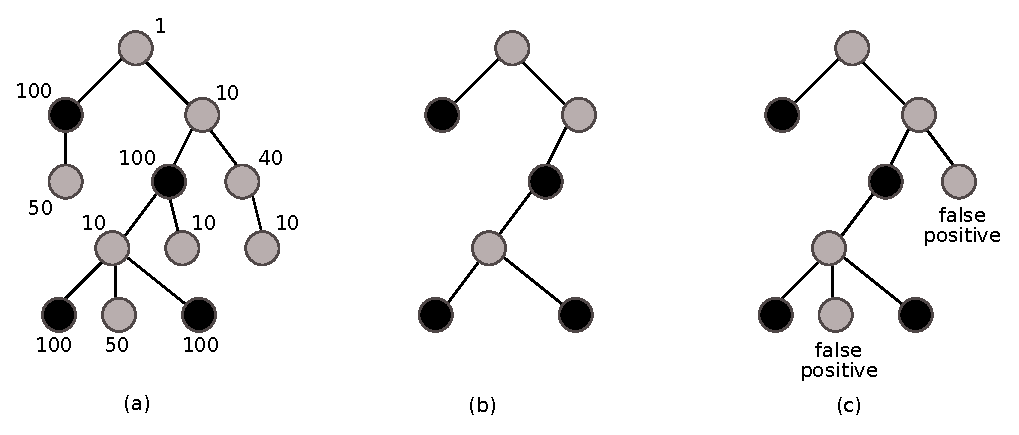
\includegraphics[width=0.95\columnwidth]{figures/hcct-example/hcct-example.eps}
\caption{\protect\label{fig:hcct-example} (a) CCT annotated with calling-context frequency counts; (b) HCCT; and (c) $(\phi,\varepsilon)$-HCCT. Hot nodes are black. In this example $N=581$, $\phi=1/10$, and $\varepsilon=1/30$: the approximate HCCT includes all contexts with frequency $\ge\lfloor\phi N\rfloor=58$  and no context with frequency $\le\lfloor(\phi-\varepsilon) N\rfloor=38$.
}
\end{center}
\end{figure}
\fi

\paragraph*{A Data Streaming Problem.} The execution trace of routine invocations and terminations can be naturally regarded as a stream of items. Each item is a triple containing routine name, call site, and event type (i.e., routine invocation or termination). Figures reported in \mytable\ref{tab:hcct-CCTsize} indicate that the number of distinct routines (i.e., the number of nodes of the call graph) is small compared to the stream length (i.e., to the number of nodes of the call tree), even for complex applications. Hence, non-contextual profilers -- such as vertex profilers -- can easily collect performance metrics for all the routines using a hash table. This may not be sustainable in the case of contextual profiling, when the number of distinct calling contexts (i.e., the number of CCT nodes) is too large and hashing would be inefficient. Motivated by the fact that execution traces are typically very long and their items (calling contexts) are taken from a large universe, we cast the problem of identifying the most frequent contexts into a data streaming setting.

In the data streaming computational model, algorithms should be able to perform near-real time analyses on massive data streams, where input data come at a very high rate and cannot be stored entirely due to their huge, possibly unbounded size~\cite{Demetrescu07,Muthukrishnan05}. This line of research has been mainly motivated by networking and database applications: for instance, a relevant IP traffic analysis task consists of monitoring the packet log over a given link in order to estimate how many distinct IP addresses used that link in a given period of time. Space-efficient data streaming algorithms can maintain a compact data structure that is dynamically updated upon arrival of new input data, supporting a variety of application-dependent queries. Approximate answers are allowed when it is impossible to obtain an exact solution using only limited space. Streaming algorithms are therefore designed to optimize space usage and update/query time while guaranteeing high solution quality.

\paragraph*{Finding Frequent Items in a Stream.} The problem of computing the HCCT online can be reconducted to the {\em frequent items} (a.k.a. heavy hitters) problem, which has been extensively studied in the data streaming model. Given a frequency threshold $\phi\in[0,1]$ and a stream of length $N$, the problem (in its simplest formulation) is to find all items that appear in the stream at least $\lfloor\phi N\rfloor$ times, i.e., having frequency $\ge\lfloor\phi N\rfloor$. For instance, for $\phi=0.1$ the problem seeks all items that appear in the stream at least $10\%$ of the times. Notice that at most $1/\phi$ items can have frequency larger than $\lfloor\phi N\rfloor$.  It can be proved that any algorithm that outputs an exact solution requires $\Omega(N)$ bits, even using randomization~\cite{Muthukrishnan05}. Note that this lower bound result extends to the problem of computing the HCCT, which thus cannot be calculated exactly in a space asymptotically smaller than the entire CCT. Hence, researchers have focused on solving an approximate version of the problem:

\begin{definition} 
{\mbox{$(\phi,\varepsilon)$-heavy hitters problem.}} Given two parameters $\phi,\varepsilon\in[0,1]$, with $\varepsilon<\phi$, an algorithm has to return all items with frequency $\ge\lfloor\phi N\rfloor$ and no item with frequency $\le\lfloor(\phi-\varepsilon) N\rfloor$.
\end{definition} 

\noindent In the approximate solution, false negatives are not allowed, i.e., all frequent items must be returned. Instead, some false positives can exist, but their actual frequency is guaranteed to be at most $\varepsilon N$-far from the threshold $\lfloor\phi N\rfloor$. For the HCCT construction, we focus on a variant of the problem where, besides returning the heavy hitters, it is necessary to estimate accurately their true frequencies, the stream length $N$ is not known in advance, and all the items in the stream have equal weight.

Counter-based streaming algorithms solve this problem by tracking a subset of items from the input and monitoring counts associated with them. For each new arrival, these algorithms decide whether to store the item or not, and, if so, what counts to associate with it. Update times are typically dominated by a small (constant) number of dictionary or heap operations. These algorithms, according to extensive experimental studies~\cite{Cormode08}, have superior performance with respect to space, running time, and accuracy compared to other classes of algorithm for $(\phi,\varepsilon)$-heavy hitters that have been proposed in the literature in the last 15 years.

\paragraph*{Approximate HCCT.} Streaming algorithms for mining frequent items can be used to solve a relaxed version of the HCCT construction problem. We thus compute an {\em Approximate Hot Calling Context Tree} that we denote by {\em $(\phi,\varepsilon)$-HCCT}, where $\varepsilon<\phi$ controls the degree of approximation:

\begin{definition}
Given a set A of $(\phi,\varepsilon)$-heavy hitters, the {\em $(\phi,\varepsilon)$-HCCT} is the minimal subtree of the CCT spanning all the nodes in A and the CCT root.
\end{definition}

\noindent A $(\phi,\varepsilon)$-HCCT contains all hot nodes (true positives), but may possibly contain some cold nodes without hot descendants (false positives). The true frequency of these false positives, however, is guaranteed to be at least $\lfloor(\phi-\varepsilon) N\rfloor$. Unlike the HCCT, a $(\phi,\varepsilon)$-HCCT is not uniquely defined, since the set of $(\phi,\varepsilon)$-heavy hitters is not unique: nodes with frequencies smaller than $\lfloor\phi N\rfloor$ and larger than $\lfloor(\phi-\varepsilon) N\rfloor$ may be either in such a set or not depending on the streaming algorithm being used. On the other hand, the HCCT is always a subtree of any $(\phi,\varepsilon)$-HCCT.

\ifdefined\noauthorea
\begin{figure}[ht]
\begin{center}
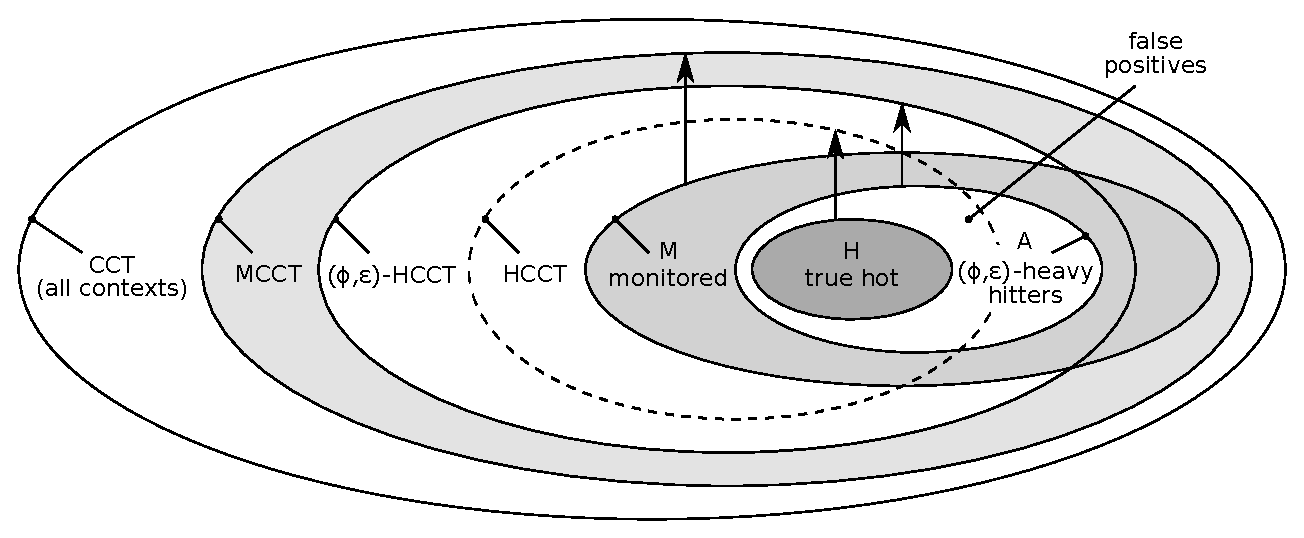
\includegraphics[width=0.95\columnwidth]{figures/hcct-venn/hcct-venn.eps}
\caption{\protect\label{fig:hcct-venn} Tree data structures and calling contexts classification. We use the graphical notation S $\uparrow$ T to indicate that T is the minimal subtree of the CCT spanning all nodes in S and their ancestors.
}
\end{center}
\end{figure}
\fi

\subsection{Algorithms}
\label{ss:hcct-algorithms}

Computing a $(\phi,\varepsilon)$-HCCT online requires extending the canonical CCT construction algorithm with an online pruning strategy, which is implicitly driven by the actions of an underlying streaming algorithm. Constructing a CCT on-the-fly during the execution of a program is a straightforward task. Let $v$ be a cursor pointer that points to the current context, i.e., to the node corresponding to the calling context of the currently active routine ($v$ is initialized to the CCT root node). At each routine invocation, the algorithm checks whether $v$ has a child associated with the called routine. If this is the case, the existing child is used and its metrics are updated, if needed. Otherwise, a new child of $v$ is added to the CCT. In both cases, the cursor is moved to the callee. Upon routine termination, the cursor is moved back to the parent node in the CCT. Note that this approach can be implemented either by instrumenting every routine call and return or by performing stack-walking if sampling is used to inhibit redundant profiling~\cite{Arnold00,Whaley00,Zhuang06}.

In order to computer the set A of $(\phi,\varepsilon)$-heavy hitters, counter-based streaming algorithms need to monitor a slightly larger set M$\,\supseteq\,$A of elements. Nodes in M$\,\setminus\,$A can be either ancestors of nodes in A and thus already in the $(\phi,\varepsilon)$-HCCT, or nodes not in the $(\phi,\varepsilon)$-HCCT; for the latter category, we have to retain information about their ancestors as well, which might not be in the $(\phi,\varepsilon)$-HCCT. We denote as MCCT the minimal subtree of the CCT spanning all the nodes in M and the CCT root. \myfigure\ref{fig:hcct-venn} graphically illustrates the relationships among all our data structures.

Our $(\phi,\varepsilon)$-HCCT construction algorithm has to maintain the MCCT dynamically while the underlying algorithm processes the execution trace and updates M. At query time, the streaming algorithm analyzes M to discard all the elements in M$\,\setminus\,$A: the MCCT is thus pruned appropriately and the $(\phi,\varepsilon)$-HCCT$\,\subseteq\,$MCCT is returned.

\paragraph*{An Example.} To understand why the heavy hitters and the approximate HCCT are not maintained directly, but derived by pruning M and MCCT, respectively, we discuss a scenario where M is larger than the number of heavy hitters. Consider the following example: the execution trace contains the initial invocation of the {\tt main} function, which in turn invokes once a routine $p$, and $N-2$ times a different routine $q$. Hence, we have three distinct calling contexts: {\tt main}, {\tt main}$\rightarrow${\tt p}, and, {\tt main}$\rightarrow${\tt q}. Assume that $N\ge 8$, $\varepsilon=1/4$, $\phi=1/2$, and that the counter-based streaming subroutine can maintain three counters, one for each calling context. Then, only context {\tt main}$\rightarrow${\tt q} has frequency larger than $\lfloor(\phi-\varepsilon)N\rfloor$ and is a $(\phi,\varepsilon)$-heavy hitter, but -- as we assumed there is room in M for all contexts -- a streaming algorithm can maintain the exact frequencies of both {\tt main}$\rightarrow${\tt p} and {\tt main}$\rightarrow${\tt q}. Since {\tt main}$\rightarrow${\tt p} has frequency 1, it would be an error returning it as a heavy hitter. For this reason, M needs to be post-processed in order to eliminate low-frequency items that may be included when there are more available counters than heavy hitters.

\paragraph*{Data Structure Operations.} At each function call, the set M of monitored contexts is updated by a counter-based streaming algorithm. When M is changed, the subtree MCCT spanning nodes in M needs to be brought up to date as well. To describe how this happens, we assume that the interface of the streaming algorithm provides two main functions:

%TODO fix alignment
%\begin{enumerate}[align=left,leftmargin=*]
\begin{description}
\item[{\tt update(x,M)}$\rightarrow\,${\tt V}] Given a calling context $x$, update M to reflect the new occurrence of $x$ in the stream (e.g., if $x$ was already monitored in M, its frequency count may be increased by one). This function might return a set V of {\em victim} contexts that were previously monitored in M and are evicted during the update (as a special case, $x$ itself may be considered as a victim if the algorithm chooses not to monitor it).
\item[{\tt query(M)}$\rightarrow\,${\tt A}] Remove low-frequency items from M and return the subset A of $(\phi,\varepsilon)$-heavy hitters (see \myfigure\ref{fig:hcct-venn}).
\end{description}
%\end{enumerate}

\ifauthorea{}{\par\begingroup \parfillskip 0pt \relax}
\noindent As with the CCT, during the construction of the MCCT we maintain a cursor pointer that points to the current calling context, creating a new node if the current context $x$ is encountered for the first time. Additionally, we prune the MCCT according to the victim contexts returned by the streaming {\tt update} operation (these contexts are no longer monitored in M). The pseudocode of the pruning algorithm is given in \myalgorithm\ref{alg:hcct-update}. Since the tree must remain connected, victims can be removed from
\ifauthorea{}{\par\endgroup}

\ifdefined\noauthorea
\begin{figure}[h!]
\IncMargin{2em}
\begin{algorithm}[H]
\LinesNumbered
\SetAlgoNoLine
\SetNlSkip{1.5em} 
\Indm\Indmm
\nonl\hrulefill\\
\KwIn{MCCT; node $x$ to be pruned.}
\KwOut{Pruned MCCT.}
\vspace{-2mm}\hrulefill\\
\Indp\Indpp
$V$ $\gets$ {\tt update}(x, M);\\
\ForEach{context $v\in V\,\backslash \{x\}$}{
    \While{$(v$ is a leaf in MCCT$)$ $\wedge$ $(v\not\in$ M$)$}{
        remove $v$ from MCCT\\
        $v$ $\gets$ parent$(v)$
    }
}
\vspace{-2mm}
\Indm\Indmm
\nonl\hrulefill\vspace{1mm}\\
\DecMargin{2em}
\caption{\label{alg:hcct-update} Online pruning algorithm for MCCT construction.}
\end{algorithm}
\end{figure}


\noindent
\fi
the MCCT only if they are leaves. Moreover, removing a victim might expose a path of unmonitored ancestors that no longer have descendants in M: these nodes are pruned as well. The node for the current context $x$ is never removed from the MCCT, even if the context is not necessarily monitored in M. This guarantees that no node in the path from the tree root to $x$ will be removed: these nodes have at least $x$ as a descendant and the leaf test (line 3 in \myalgorithm\ref{alg:hcct-update}) will always fail.
A similar pruning strategy can be used to compute the $(\phi,\varepsilon)$-HCCT from the MCCT. The streaming {\tt query} operation is first invoked on M, returning the support A of the $(\phi,\varepsilon)$-HCCT. All MCCT nodes that have no descendant in A are then removed, following bottom-up path traversals as in the prune operation.

\ifx\noauthorea\undefined
\begin{figure}[ht]
\caption{\label{alg:hcct-update} Online pruning algorithm for MCCT construction.\hfill}
\begin{small}
\begin{minipage}{0.9\textwidth}
\hrulefill\\
\textbf{Input}: {MCCT; node $x$ to be pruned.}\\
\textbf{Output}: {Pruned MCCT.}

\vspace{-1mm}
\hrulefill\\
1. ~~ $V$ $\gets$ {\tt update}(x, M);\\
2. ~~ \textbf{foreach} context $v\in V\,\backslash \{x\}$ \textbf{do}\\
3. ~~ ~~~~ \textbf{while} $(v$ is a leaf in MCCT$)$ $\wedge$ $(v\not\in$ M$)$ \textbf{do}\\
4. ~~ ~~~~ ~~~~ remove $v$ from MCCT\\
5. ~~ ~~~~ ~~~~ $v$ $\gets$ parent$(v)$\\
6. ~~ ~~~~ \textbf{end}\\
7. ~~ \textbf{end}

\vspace{-1mm}
\hrulefill
\vspace{-2mm}
\end{minipage}
\end{small}
\end{figure}
\fi

%Algorithmic details on updating and querying M and MCCT are given in \mysection\ref{ss:hcct-algorithms}.

%\subsection{Implementation}

\subsection{Comparison with Related Work}

\subsection{Discussion}

% dire dello spazio asintoticamente minore
\newpage
\section{Intraprocedural Profiling}

{\em Path profiling} is a powerful {\em intraprocedural} methodology for identifying performance bottlenecks in a program, and has received considerable attention in the last 15 years for its practical relevance. The well-known Ball and Larus numbering algorithm~\cite{Ball96} can efficiently encode {\em acyclic} paths that are taken across the control-flow graph of a function. Previous attempts to extend it to {\em cyclic} paths, as spanning multiple loop iterations, to capture more optimization opportunities, are based on rather complex algorithms that incur severe performance overheads even for short cyclic paths. In this thesis we present a new, data-structure based approach to {\em multi-iteration} path profiling built on top of the original Ball-Larus numbering technique. Starting from the observation that a cyclic path can be described as a concatenation of Ball-Larus acyclic paths, we show how to accurately profile all executed paths obtained as a concatenation of up to $k$ Ball-Larus paths, where $k$ is a user-defined parameter.

%{\em Path profiling} is a powerful {\em intraprocedural} methodology for identifying performance bottlenecks in a program, and has received considerable attention in the last 15 years for its practical relevance. The well-known Ball and Larus algorithm~\cite{Ball96} for {\em intraprocedural} path profiling can efficiently encode {\em acyclic} paths that are taken across the control-flow graph of a function. Previous attempts to extend it to encode {\em cyclic} paths, and thus to span multiple loop iterations in order to capture more optimization opportunities, are based on rather complex algorithms that incur severe performance overheads even for short cyclic paths. In this thesis we present a new, data-structure based approach to {\em multi-iteration} path profiling built on top of the original Ball-Larus numbering technique. Starting from the observation that any cyclic path can be described as a concatenation of Ball-Larus acyclic paths, we show how to accurately profile all executed paths obtained as a concatenation of up to $k$ Ball-Larus paths, where $k$ is a user-defined parameter.

%We provide examples showing that this method can reveal optimization opportunities that acyclic-path profiling would miss, and we present an extensive experimental investigation on a large variety of Java benchmarks in the Jikes RVM. Experiments show that our approach can be even faster than a hash table-based implementation of the Ball-Larus algorithm due to fewer operations on smaller tables, producing compact representations of cyclic paths even for large values of $k$.

\subsection{Motivation and Contributions}

Path profiling associates performance metrics, usually frequency counters, to paths taken in the control flow graph of a routine. Identifying the hottest paths can direct optimizations to portions of the code where most resources are consumed, often yielding significant speedups. For instance, trace scheduling can improve performance by increasing instruction-level parallelism along frequently executed paths~\cite{Fisher81,Young98}. Although basic block and edge profiles are inexpensive and widely available, they do not always correctly predict frequencies of overlapping paths. 

The seminal paper by Ball and Larus~\cite{Ball96} introduced a simple and elegant path profiling technique. The main idea was to implicitly number all possible acyclic paths in the control flow graph so that each path is associated with a unique compact path identifier (ID). The authors showed that path IDs can be efficiently generated at runtime and can be used to update a table of frequency counters. Although in general the number of acyclic paths may grow exponentially with the graph size, in typical control flow graphs this number is usually small enough to fit in current machine word-sizes, making this approach very effective in practice.

While the original Ball-Larus approach was restricted to acyclic paths obtained by cutting paths at loop back edges, profiling paths that span consecutive loop iterations is a desirable, yet difficult, task that can yield better optimization opportunities. Consider, for instance, the problem of eliminating redundant executions of instructions, such as loads and stores~\cite{Bodik99}, conditional jumps~\cite{Bodik97}, expressions~\cite{Bodik98,Bodik04}, and array bounds checks~\cite{Bodik00}. A typical situation is that the same instruction is redundantly executed at each loop iteration, which is particularly common for arithmetic expressions and load operations~\cite{Bodik04,Bodik99}. To identify such redundancies, paths that extend across loop back edges need to be profiled. Another application is trace scheduling~\cite{Young98}: if a frequently executed cyclic path is found, compilers may unroll the loop and perform trace scheduling on the unrolled portion of code. Tallam {\em et al.}~\cite{Tallam04} provide a comprehensive discussion of the benefits of multi-iteration path profiling.

Different authors have proposed techniques to profile cyclic paths by modifying the original Ball-Larus path numbering scheme in order to identify paths that extend across multiple loop iterations~\cite{Tallam04,Roy09,Li12}. Unfortunately, all known solutions require rather complex algorithms that incur severe performance overheads even for short cyclic paths, leaving the interesting open question of finding simpler and more efficient alternative methods.

\paragraph*{Contributions.}

\subsection{Approach}

\subsection{Algorithms}

%\subsection{Implementation}

\subsection{Comparison with Related Work}

\subsection{Discussion}
\fi

\section{Conclusions}
Low-overhead profiling mechanisms are a key ingredient for effective adaptive optimization in a runtime system. For some classes of profiling information, the sheer size of the domain might require an analysis routine to maintain a large amount of data in main memory, resulting in a performance penalty from poor access locality or even the exhaustion of available resources. This is the case of context-sensitive profiling, for which we have introduced a new data structure, the HCCT, that can be constructed online in small space with strong guarantees in terms of accuracy and recall. We present and evaluate an implementation of a HCCT profiler in \mysection\ref{ss:hcct-eval}.

Another example is cyclic-path profiling, for which extant techniques fail to scale as enumerating paths explicitly results into an explosion in the number of possible sequences already for a few loop iterations. We have presented an encoding scheme based on a prefix forest, the \kipf, obtainable on demand from an intermediate data structure, the \ksf, that can be constructed online efficiently. We describe and evaluate an implementation of this technique in Jikes RVM in \mysection\ref{ss:kblpp-eval}.
% !TEX root = thesis.tex

\chapter{Continuous Program Optimization Techniques}
\label{ch:continuous}

In this chapter, we focus on a fundamental aspect for deploying adaptive optimization techniques in runtime systems: the {\em On-Stack Replacement} (OSR) problem. OSR consists in dynamically transferring execution between different versions of a function at run time. Modern virtual machines implement OSR to {\em continuously} optimize a program as it executes, for instance by interrupting a long-running function and recompiling it at a higher optimization level, or by replacing a function version with another when a speculative assumption made during its compilation no longer holds.

In the first part of the chapter, we present a platform-independent framework for OSR that introduces novel ideas and combines features of existing techniques that no previous solution provided simultaneously. In particular, we introduce a {\em compensation code} abstraction that increases the flexibility of OSR mechanisms, and we present an OSR implementation for the LLVM MCJIT compiler that allows OSR to happen at arbitrary locations in a function.

In the second part, we make a first step towards a provably sound methodological framework for OSR. We formalize the concept of {\em multi-version program}, and we identify sufficient conditions for the correctness of an OSR transition. We also devise an algorithm for automatically generating compensation code possibly required to realign program state in the presence of several common compiler optimizations.

\input{osrkit}
\section{Proving On-Stack Replacement Sound}

On-stack Replacement is employed in modern adaptive compilation systems to dynamically switch between different versions of a function depending on program's run-time state. Traditionally, code optimizers are responsible for marking the points where such transitions can take place, and generating required meta-data or ad-hoc code to get the program state to a correct resumption point. OSR is usually at the core of large and complex JIT compilers employed by popular production virtual machines. Indeed, the engineering effort to integrate this technique in a language runtime can be daunting, making it rarely accessible to the research community.

\paragraph*{Contributions.} In this thesis we investigate how to provide VM builders with a rich ``menu'' of possible program points where OSR can safely occur, relieving code optimizers from the burden of generating all the required machinery to realign the program state during an OSR transition.

To capture OSR in its full generality, we define a notion of {\em multi-program}, which is a collection of different versions of a program along with support to dynamically transfer execution between them. Execution in a multi-program starts from a designated base version. At any time, an oracle decides whether execution should continue in the current version, or an OSR should divert it to a different version, modeling any conceivable OSR-firing strategy. One of the goals of our work is to characterize sufficient conditions for a multi-program to be {\em deterministic}, yielding the same result regardless of the oracle's decisions. This captures the intuitive idea that any sequence of OSR transitions is {\em correct} if it does not alter the intended semantics of a program.

We distill the essence of OSR to a simple imperative calculus with an operational semantics. Using program bisimulation, we prove that an OSR can correctly divert execution from one program version to the other if they are {\em live-variable bisimilar}, i.e., the live variables they have in common at any corresponding execution states are equal. As prominent examples of how bisimulation can be used to prove this property, we consider classic optimizations that eliminate or move code around, such as dead code elimination, constant propagation, and code hoisting. We show how to construct OSR machinery by devising an algorithm that automatically generates compensation code to reconstruct the values of variables that are live in the OSR target, but not in the source.

\subsection{Language Syntax and Semantics}
\label{ss:osr-language-framework}
Our discussion is based on a minimal imperative programming whose syntax is reported \ifauthorea{below}{in \myfigure\ref{fig:osr-program-syntax}}. In this section we introduce some basic definitions used in our representation of programs, and provide a big-step semantics for the language.

%\subsection{Language Framework}

%In this section we introduce some basic definitions used in our representation of programs and transformations. In particular, we provide a syntax and a big-step semantics for a simple imperative language, and introduce means for reasoning about program properties using computation tree logic operators and for describing program transformations through rewrite rules with side conditions.

%\subsubsection*{Program Syntax and Semantics}

%Our discussion is based on a minimal imperative programming language with instructions and expressions with the syntax \ifauthorea{below}{in \myfigure\ref{fig:osr-program-syntax}}.

\ifdefined\noauthorea
\begin{figure}[t]
\fi
\noindent
\begin{small}
$
\begin{array}{rcl}
\texttt{$Instr$} & ::= & \hphantom{\texttt{| }}\texttt{$Var$ := $Expr$} \\
& & \texttt{| if ( $Expr$ ) goto $Num$} \\
& & \texttt{| goto $Num$} \\
& & \texttt{| skip} \\
& & \texttt{| abort} \\
& & \texttt{| in $Var\cdots Var$} \\ 
& & \texttt{| out $Var\cdots Var$} \\
\texttt{ $Expr$ } & ::= & \texttt{$Num$ | $Var$ | $Expr$ + $Expr$ | $\ldots$ } \\
\texttt{ $Var$ } & ::= & \texttt{X | Y | Z | $\ldots$} \\
\texttt{ $Num$ } & ::= & \texttt{$\ldots$ | -2 | -1 | 0 | 1 | 2 | $\ldots$} \\
\end{array}
$
\end{small}
\ifdefined\noauthorea
\caption{\label{fig:osr-program-syntax}Program Syntax}
\end{figure}
\fi

\begin{definition}[Program]
\label{de:program}
A program is a sequence of instructions the form:
\vspace{-3mm}
\begin{equation*}
\pi=\langle I_1, I_2, \ldots, I_n \rangle\in Prog = \bigcup_{i=2}^{\infty} Instr^{i}
\vspace{-4mm}
\end{equation*}
where: 

\begin{itemize}[itemsep=3pt,parsep=0pt,topsep=3pt]
%\item $Instr$ is defined by the syntax of Figure~\ref{fi:program-syntax}
\item \texttt{$I_i\in Instr$} is the $i$-th instruction of the program, indexed by program point \texttt{$i\in[1,n]$}
\item \texttt{$I_1$ $=$ in $\cdots$} is the initial instruction
\item \texttt{$\forall i\in[2,n-1]:$ $I_i$ $\neq$ in $\cdots$ $\wedge$ $I_i$ $\neq$ out $\cdots$}
\item \texttt{$I_n$ $=$ out $\cdots$} is the final instruction
\end{itemize}
\end{definition}

\noindent Instruction \texttt{in}, which must appear at the beginning of a program, specifies the variables that must be defined prior to entering the program. Similarly, \texttt{out} occurs at the end and specifies the variables that are returned as output. 

By \texttt{e[x]} we indicate that \texttt{x} is a variable of expression \texttt{e}\,$\in Expr$. We also denote by $vars($\texttt{e}$)$ the set of variables that occur in expression \texttt{e}. By $|\pi|=n$ we indicate the number of instructions in $\pi=\langle I_1, I_2, \ldots, I_n \rangle$.

\begin{definition}[Memory Store]
A {\em memory store} is a total function $\sigma:Var\rightarrow \mathbb{Z}\cup\{\bot\}$ that associates integer values to defined variables, and $\bot$ to undefined variables. We denote by $\Sigma$ the set of all possible memory stores. 
\end{definition}

\noindent By $\sigma[\wx\gets v]$ we denote the same function as $\sigma$, except that $\wx$ takes value $v$. Furthermore, for any $A\subseteq Var$, $\sigma\vert_{A}$ denotes $\sigma$ restricted to the variables in $A$, i.e., $\sigma\vert_{A}(\wx)=\sigma(\texttt{x})$ if $\wx\in A$ and $\sigma\vert_{A}(\wx)=\bot$ if $\wx\not\in A$. 

\begin{definition}[Program State]
\label{de:prog-state}
The {\em state} of a program $\pi=\langle I_1, I_2, \ldots, I_n \rangle$ is described by a pair $(\sigma,l)$, where $\sigma$ is a memory store and $l\in [1,n]$ is the program point of the next instruction to be executed. We denote by $State=\Sigma\times \mathbb{N}$ the set of all possible program states.
\end{definition}

\noindent We provide a big-step semantics using transition relation $\trans_{\pi}\:\subseteq State\times State$, which specifies how a single instruction of a program $\pi$ affects its state. Our description relies on relation $\Downarrow\subseteq(\Sigma\times Expr)\times \mathbb{Z}$ to describe how expressions are evaluated in a given memory store.


\begin{definition}[Big-Step Transitions]
\label{de:transitions}
%For any program $\pi$, relation $\Rightarrow_{\pi}\subseteq State\times State$ is defined as follows, with meta-variables $\texttt{x}, \texttt{y}\in Var$, $\texttt{e}\in Expr$, and $\texttt{m}\in Num$:
For any program $\pi$, we define relation $\Rightarrow_{\pi}\:\subseteq State\times State$ as follows, with meta-variables $\texttt{x}, \texttt{y}\in Var$, $\texttt{e}\in Expr$, and $\texttt{m}\in Num$:

\begin{small}

% asgn
\begin{equation}
\label{eq:asgn-sem}
\frac
{I_l=\texttt{x:=e} ~~ \wedge ~~ (\sigma, \texttt{e}) \Downarrow v}
{(\sigma, l)\Rightarrow_{\pi} (\sigma[\wx\gets v], l+1)}
\end{equation}
% if (0)
\vspace{0.5mm}
\begin{equation}
\label{eq:ifz-sem}
\frac
{I_l=\texttt{if (e) goto m} ~~ \wedge ~~ (\sigma, \texttt{e}) \Downarrow 0}
{(\sigma, l)\Rightarrow_{\pi} (\sigma, l+1)}
\end{equation}
% if (!0)
\vspace{0.5mm}
\begin{equation}
\label{eq:ifnz-sem}
\frac
{I_l=\texttt{if (e) goto m} ~~ \wedge ~~ (\sigma, \texttt{e}) \Downarrow v ~~~ \wedge ~~~ v\neq 0}
{(\sigma, l)\Rightarrow_{\pi} (\sigma, \texttt{m})}
\end{equation}
% goto
\vspace{0.5mm}
\begin{equation}
\label{eq:goto-sem}
\frac
{I_l=\texttt{goto m}}
{(\sigma, l)\Rightarrow_{\pi} (\sigma, \texttt{m})}
\end{equation}
% skip
\vspace{0.5mm}
\begin{equation}
\label{eq:skip-sem}
\frac
{I_l=\texttt{skip}}
{(\sigma, l)\Rightarrow_{\pi} (\sigma, l+1)}
\end{equation}
% in
\vspace{0.5mm}
\begin{equation}
\label{eq:in-sem}
\frac
{I_1=\texttt{in x y}~\cdots ~~ \wedge ~~~ \sigma(\texttt{x})\neq\bot ~~~ \wedge ~~~ \sigma(\texttt{y})\neq\bot ~~~ \wedge ~~~ \cdots }
{(\sigma, 1)\Rightarrow_{\pi} (\sigma, 2)}
\end{equation}
% out
%\vspace{0.5mm}
\begin{equation}
\label{eq:out-sem}
\frac
{I_n=\texttt{out x y}~\cdots ~~ \wedge ~~~ \sigma(\texttt{x})\neq\bot ~~~ \wedge ~~~ \sigma(\texttt{y})\neq\bot ~~~ \wedge ~~~ \cdots }
{(\sigma, n)\Rightarrow_{\pi} (\sigma\vert_{\{\texttt{x}, \texttt{y}, \cdots\}}, n+1)}
\end{equation}

\end{small}

\end{definition}

\noindent For a transition to apply, we implicitly assume that $I_l$ is defined, i.e., $l\in[1,n]$. 
\ifx\noauthorea\undefined
Notice that we intentionally do not provide any transition rule for {\tt abort} instructions, providing explicit means to let a program have undefined semantics. This might be useful in supporting unsound speculative optimizations.
\fi

\begin{definition}[Program Semantic Function]
\label{de:program-semantics}
%The semantic function $\mysem{\pi}:\Sigma \rightarrow \Sigma$ of a program $\pi$ is defined as:
We define the semantic function $\mysem{\pi}:\Sigma \rightarrow \Sigma$ of a program $\pi$ as: 
\begin{gather*}
\forall \sigma\in\Sigma: ~~ \mysem{\pi}(\sigma)=\sigma'~~%\vert_{\{\wx\,:\,I_{n}={\tt out}~\cdots~\wx~\cdots\}} ~~ \\ 
\Longleftrightarrow ~~ (\sigma,1) \Rightarrow^{*}_{\pi} (\sigma',|\pi|+1)
\end{gather*}
where $\Rightarrow^{*}_{\pi}$ is the transitive closure of $\Rightarrow_{\pi}$.
\end{definition}

\noindent Note that a program has undefined semantics if its execution on a given store does not reach the final \texttt{out} instruction. This accounts for infinite loops, abort instructions, exceptions, and ill-defined programs or input stores. 

We define the notion of program semantic equivalence as follows:

\begin{definition}[Program Equivalence]
\label{de:semantic-equivalence}
Two programs $\pi_1$ and $\pi_2$ are {\em semantically equivalent} iff $\mysem{\pi_1}=\mysem{\pi_2}$.
\end{definition}

\noindent A notion that will be useful in proving correctness in our framework is that of {\em trace} of a transition system:

\begin{definition}[Traces]
\label{de:exec-trace}
A {\em trace} in a transition system $(S,$ $R\subseteq S^2)$ starting from $s\in S$ is a sequence $\tau=\langle s_0,s_1,\ldots,$ $s_i,\ldots\rangle$ such that $s_0=s$ and $\forall i\ge 0:~s_i\in\tau ~ \wedge ~ s_i~R~s_{i+1}$ $\Longleftrightarrow s_{i+1}\in\tau$. By ${\cal T}_{R,s}$ we denote the system of all traces of $(S,R\subseteq S^2)$ starting from $s$. By $\tau[i]$ we denote the $i$-th state of $\tau$, i.e., $\tau[i]=s_i$. Furthermore, if trace $\tau$ is finite then $|\tau|$ denotes the index of its final state, i.e., $\tau=\langle s_0,s_1,\ldots,s_{|\tau|}\rangle$, otherwise $|\tau|=\infty$. Finally, $dom(\tau)=\{i:s_i\in\tau\}$ denotes the set of indices of states in $\tau$.
\end{definition}

\noindent Notice that, since $\Rightarrow_{\pi}$ is deterministic in our language, then for any initial store $\sigma$, the system of traces ${\cal T}_{\Rightarrow_{\pi},(\sigma,1)}$ of the execution transition system $(Store,\Rightarrow_{\pi})$ contains a single trace, which we denote by $\tau_{\pi\sigma}$.

Finally, we provide a formal definition of control flow graph, which will be useful in defining computation tree logic operators for reasoning on program properties:

\begin{definition}[Control Flow Graph]
\label{de:cfg}
%The {\em control flow graph} G for a program $\pi=\langle I_1, I_2, \ldots, I_n \rangle$ is described by a pair $(V,E)$ where $V = \{ I_1, I_2, \ldots, I_n \}$ and $E = \{(I_i, I_{i+1})\:|\: I_i \neq \textsf{abort} \wedge I_i \neq \textsf{goto m}, \!\textsf{ m}\in Num \}\;\cup\;\{(I_i, I_m)\:|\: I_i = \textsf{goto m} \vee I_i = \textsf{if (e) goto m}, \!\textsf{ m}\in Num, \!\textsf{ e}\in Expr \}$.
%The {\em control flow graph} G for a program $\pi=\langle I_1, I_2, \ldots, I_n \rangle$ is described by a tuple $\langle V, I: V\rightarrow Num, E \subseteq V\times V\rangle$ where:
The {\em control flow graph} $G$ for a program $\pi=\langle I_1, I_2, \ldots, I_n \rangle$ is described by a pair $(V, E \subseteq V\times V)$ where:
%\begin{equation*}
\begin{align*}
V &= \{ I_1, I_2, \ldots, I_n \} \\
%I(v) &= \{ i | v = I_i, v\in V\} \\
E &= \{(I_i, I_{i+1})\:|\: I_i \neq \textsf{abort} \wedge I_i \neq \textsf{goto m}, \!\textsf{ m}\in Num \} \\
&\cup\;\{(I_i, I_m)\:|\: I_i = \textsf{goto m} \vee I_i = \textsf{if (e) goto m}, \!\textsf{ m}\in Num, \!\textsf{ e}\in Expr \}.
\end{align*}
%\end{equation*}
%\noindent We also define an auxiliary function $I: V\rightarrow Num$ that returns the $i$-th index in $\pi$ of an instruction $v\in V$.
\end{definition}
\subsubsection*{Reasoning about Program Properties}

\subsection{On-Stack Replacement Framework}

OSR consists in dynamically transferring execution from a point $l$ in a program $\pi$ to a point $l'$ in a program $\pi'$ so that execution can transparently continue from $\pi'$ without altering the original intended semantics of $\pi$. To model this behavior, we assume there exists a function that maps each point $l$ in $\pi$ where OSR can safely be fired to the corresponding point $l'$ in $\pi'$ from which execution can continue.
As we observed in \mysection\ref{ss:osr-llvm-approach}, the OSR practice often makes the conservative assumption that $\pi'$ can always continue from the very same memory store as $\pi$. However, this assumption may reduce the number of points where sound OSR transitions can be fired. To overcome this limitation and support more aggressive OSR transitions, our model includes a {\em store compensation code} $\chi$ to be executed during an OSR transition from point $l$ in $\pi$ to point $l'$ in $\pi'$. The goal of the compensation code is to fix the memory store of $\pi$ at $l$ so that execution can safely continue in $\pi'$ from $l'$ with the fixed store. Note that, if no compensation is needed for an OSR transition, $\mysem{\chi}$ is simply the identity function. We formalize these concepts in the next sections.

\subsubsection{OSR Mappings}
\label{ss:osr-mapping}

The machinery required for performing OSR transitions between two programs can be modeled as an {\em OSR mapping}:

\begin{definition}[OSR Mapping]
\label{de:osr-mapping}
For any $\pi,\pi'\in Prog$, an {\em OSR mapping} from $\pi$ to $\pi'$ is a (possibly partial) function
$\mu_{\pi\pi'}:[1,|\pi|]\rightarrow [1,|\pi'|]\times Prog$ such that:
\begin{gather*}
\forall \sigma\in\Sigma, \forall s_i=(\sigma_i,l_i)\in\tau_{\pi\sigma}~\text{s.t.}~l_i\in dom(\mu_{\pi\pi'}),~\\
\exists \sigma'\in\Sigma, \exists s_j=(\sigma_j,l_j)\in\tau_{\pi'\sigma'}~\text{s.t.}~\\
\mu_{\pi,\pi'}(l_i)=(l_j,\chi)~\wedge~\mysem{\chi}(\sigma_i\vert_{\live(\pi,l_i)})=\sigma_j\vert_{\live(\pi',l_j)}
\end{gather*}
We say that the mapping is {\em strict} if $\sigma'=\sigma$. We denote by $OSRMap$ the set of all possible OSR mappings between any pair of programs.
\end{definition}

\noindent Intuitively, an OSR mapping provides the information required to transfer execution from any realizable state of $\pi$, i.e., an execution state that is reachable from some initial store by $\pi$, to a realizable state of $\pi'$. Notice that this definition is rather general, as a non-strict mapping allows execution to be transferred to a program $\pi'$ that is {\em not} semantically equivalent to $\pi$. For instance, $\pi'$ may contain speculatively optimized code, or just some optimized fragments of $\pi$~\cite{Guo11, Bala00, Gal09}. In those scenarios, one typically assumes that execution in $\pi'$ can be invalidated by performing an OSR transition back to $\pi$ or to some other recovery program. We also observe that \mydefinition\ref{de:osr-mapping} uses a weak notion of store equality restricted to live variables. To simplify the discussion, we assume that the memory store is only defined on scalar variables (we address extensions to memory \mytt{load} and \mytt{store} instructions in Section\missing). Hence, the behavior of a program only depends on the content of its live variables, as stated in the following lemma:

\begin{lemma}
\label{le:only-live-count}
For any program $\pi\in Prog$, any $\sigma,\sigma'\in\Sigma$, and any $l,l'\in \mathbb{N}$, it holds: 
$$
(\sigma,l)\Rightarrow_{\pi}(\sigma',l') ~~ \Longleftrightarrow ~~ (\sigma\vert_{\live(\pi,l)},l)\Rightarrow_{\pi}(\sigma'\vert_{\live(\pi,l')},l')
$$
\end{lemma}

\noindent Notice that $dom(\mu_{\pi\pi'})\subseteq [1,|\pi|]$ is the set of all possible points in $\pi$ where OSR transitions to $\pi'$ can be fired. If $\mu_{\pi\pi'}$ is partial, then there are points in $\pi$ where OSR cannot be fired. In Section\missing, we discuss an algorithm whose goal is to minimize the number of these points.


\subsubsection{OSR Mapping Generation Algorithm}
We now discuss an algorithm that, given a program $\pi$ and a rewrite rule $T$, generates:
\begin{enumerate}[itemsep=0pt,parsep=3pt]
 \item a program $\pi'=\mysem{T}(\pi)$;
 \item an OSR mapping $\mu_{\pi\pi'}$ from $\pi$ to $\pi'$;
 \item an OSR mapping $\mu_{\pi'\pi}$ from $\pi'$ to $\pi$.
\end{enumerate}

\noindent Mappings $\mu_{\pi\pi'}$ and $\mu_{\pi'\pi}$ produced by the algorithm are based on compensation code that runs in $O(1)$ time and support bidirectional OSR between $\pi$ and $\pi'$, enabling invalidation and deoptimization. The algorithm, which we call \osrtrans, is shown \ifauthorea{below}{in \myalgorithm\ref{alg:osr-trans}}. In Section\missing, we prove that the algorithm is correct under the sufficient condition that variables that are live at corresponding points in the original and rewritten program contain the same values.

%% OSR_trans
\ifdefined\noauthorea
\begin{figure}[ht!]
\IncMargin{2em}
\begin{algorithm}[H]
\DontPrintSemicolon
\LinesNumbered
\SetAlgoNoLine
\SetNlSkip{1em} 
\Indm\Indmm
\hrulefill\\
%$\mathbf{algorithm} \> \> \osrtrans$($\pi, T$)$\rightarrow$($\pi',\mu_{\pi\pi'},\mu_{\pi'\pi}$):\;
%\vspace{1mm}
\KwIn{Program $\pi$, transformation $T$.}
\KwOut{Program $\pi'$, OSR mappings $\mu_{\pi\pi'}$ and $\mu_{\pi'\pi}$.}
\nonl\vspace{-2mm}\hrulefill\\
\nonl$\mathbf{algorithm} \> \> \osrtrans$($\pi, T$)$\rightarrow$($\pi',\mu_{\pi\pi'},\mu_{\pi'\pi}$):\;
\everypar={\nl}
\Indp\Indpp
\vspace{1mm} $(\pi',\Delta,\Delta')\gets \texttt{apply}(\pi,T)$\;
\ForEach{$l\in dom(\Delta)$}{
    $\chi\gets\buildcomp(\pi,l,\pi',\Delta(l))$\;
    \lIf{$\chi\neq~\mundef$}{
	$\mu_{\pi\pi'}(l)\gets(\Delta(l),\chi)$
    }
}
\ForEach{$l'\in dom(\Delta')$}{
    $\chi\gets\buildcomp(\pi',l',\pi,\Delta'(l'))$\;
    \lIf{$\chi\neq~\mundef$}{
	$\mu_{\pi'\pi}(l')\gets(\Delta'(l'),\chi)$
    }
}
\Return{$(\pi',\mu_{\pi\pi'},\mu_{\pi'\pi})$}\;
\vspace{-2mm}
\Indm\Indmm
\nonl\hrulefill\vspace{1mm}\\
\DecMargin{0.5em}
%\caption{\label{alg:osr-trans} OSR mapping construction algorithm.}
\caption{\label{alg:osr-trans} \osrtrans\ algorithm for OSR mapping construction. Functions $\Delta$ and $\Delta'$ are used to map OSR program points between $\pi$ and $\pi'$ (and viceversa).}
\IncMargin{0.5em}
%\DecMargin{0.5em}
\end{algorithm} 
\end{figure}

\else
\begin{figure}
\noindent
\begin{small}
\hphantom{xxx} $\textbf{algorithm}~\osrtrans(\pi, T)\rightarrow (\pi',\mu_{\pi\pi'},\mu_{\pi'\pi})$ \\
1.\hphantom{0} ~~ ~~~~ $(\pi',\Delta,\Delta')\gets \texttt{apply}(\pi,T)$ \\
2.\hphantom{0} ~~ ~~~~ $\textbf{for each}~l\in dom(\Delta)~\textbf{do}$ \\
3.\hphantom{0} ~~ ~~~~ ~~~~ $\chi\gets\buildcomp(\pi,l,\pi',\Delta(l))$ \\
4.\hphantom{0} ~~ ~~~~ ~~~~ $\textbf{if}~\chi\neq~\mundef~\textbf{then}~\mu_{\pi\pi'}(l)\gets(\Delta(l),\chi)$ \\
5.\hphantom{0} ~~ ~~~~ $\textbf{done}$\\
6.\hphantom{0} ~~ ~~~~ $\textbf{for each}~l'\in dom(\Delta')~\textbf{do}$ \\
7.\hphantom{0} ~~ ~~~~ ~~~~ $\chi\gets\buildcomp(\pi',l',\pi,\Delta'(l'))$ \\
8.\hphantom{0} ~~ ~~~~ ~~~~ $\textbf{if}~\chi\neq~\mundef~\textbf{then}~\mu_{\pi'\pi}(l')\gets(\Delta'(l'),\chi)$ \\
9.\hphantom{0} ~~ ~~~~ $\textbf{done}$\\
10. ~~ ~~~~ $\textbf{return}~(\pi',\mu_{\pi\pi'},\mu_{\pi'\pi})$ \\
\end{small}
\caption{\osrtrans\ algorithm for OSR mapping construction. Functions $\Delta$ and $\Delta'$ are used to map OSR program points between $\pi$ and $\pi'$ (and viceversa).}
\label{alg:osr-trans}
\end{figure}
\fi


%% build_comp
\ifdefined\noauthorea
\begin{figure}[ht!]
\IncMargin{2em}
\begin{algorithm}[H]
\DontPrintSemicolon
\LinesNumbered
\SetAlgoNoLine
\SetNlSkip{1em} 
\Indm\Indmm
\hrulefill\\
%$\mathbf{algorithm} \> \> \osrtrans$($\pi, T$)$\rightarrow$($\pi',\mu_{\pi\pi'},\mu_{\pi'\pi}$):\;
%\vspace{1mm}
\KwIn{Program $\pi$, point $l$, program $\pi'$, point $l'$.}
\KwOut{Store compensation code $\chi$.}
\nonl\vspace{-2mm}\hrulefill\\
%$\textbf{algorithm}~\buildcomp(\pi, l, \pi', l')\rightarrow \chi$ \\
\nonl$\mathbf{algorithm} \> \> \buildcomp$:\;
\everypar={\nl}
\Indp\Indpp
\vspace{1mm} $\chi\gets \textbf{in}~x_1~x_2~\cdots~x_k\,:\,\forall i\in[1,k]:\pi,l \models \live(x_i)$\;
mark all program points of $\pi'$ as unvisited\;
$\mathbf{try}$\;
\Indp
\ForEach{$\wx:~\pi',l'\models\live(\wx)\wedge\pi,l\models\neg\live(\wx)$}{
    $\chi \gets \chi \cdot \reconstruct(\wx, \pi, l, \pi', l', l')$\;
}
\Indm
$\mathbf{catch}$\;
\Indp
$\mathbf{return}~\mundef$\;
\Indm
$\chi\gets \chi\cdot\textbf{out}~x_1~x_2~\cdots~x_k:\forall i\in[1,k]:\pi',l'\models \live(x_i)$\;
\Return{$\chi$}\;
\vspace{-2mm}
\Indm\Indmm
\nonl\hrulefill\vspace{1mm}\\
\IncMargin{1.5em}
\caption{\label{alg:osr-build-comp} \buildcomp\ algorithm for compensation code construction.}
\DecMargin{1.5em}
\end{algorithm} 
\end{figure}

\else
\begin{figure}
\noindent
\begin{small}
\algmissing \\
\end{small}
\caption{\buildcomp\ algorithm for compensation code construction.}
\label{alg:osr-build-comp}
\end{figure}
\fi


\paragraph*{\texttt{OSR\_trans}:} the algorithm relies on two subroutines: \apply\ and \buildcomp. Procedure \apply\ takes as input a program $\pi$ and a program rewriting function $T$, and returns a transformed program $\pi'$ and two functions $\Delta:[1,|\pi|]\rightarrow [1,|\pi'|]$, $\Delta':[1,|\pi'|]\rightarrow [1,|\pi|]$ that map OSR program points between $\pi$ and $\pi'$. 
Algorithm \buildcomp\ (shown \ifauthorea{above}{in \myalgorithm\ref{alg:osr-build-comp}}) takes as input $\pi$, $l$, $\pi'$, $l'$ and aims to build a {\em store compensation code} $\chi$ that allows firing an OSR from $\pi$ at $l$ to $\pi'$ at $l'$. \osrtrans\ first calls \apply\ and then uses \buildcomp\ on $\pi$, $\pi'$, $\Delta$, $\Delta'$ to build OSR mappings $\mu_{\pi\pi'},\mu_{\pi'\pi}$. Lines 2--5 build the forward mapping $\mu_{\pi\pi'}$ from $l$ in $\pi$ to $\Delta(l)$ in $\pi'$, while lines 6--9 build the backward mapping $\mu_{\pi'\pi}$ from $l'$ in $\pi'$ to $\Delta'(l')$ in $\pi$. If any of the live variables at the OSR destination cannot be guaranteed to be correctly assigned, no entry is created in $\mu_{\pi\pi'}$ or $\mu_{\pi'\pi}$ for the OSR origin point (lines 4 and 8). Hence, those points will not be eligible for OSR transitions. In Section \missing\ we will analyze experimentally the fraction of points for which a compensation code can be created by algorithm \buildcomp\ in a variety of prominent benchmarks.

\paragraph*{\texttt{build\_comp}:} the algorithm (\ifauthorea{shown below}{shown in \myalgorithm\ref{alg:osr-build-comp}}) generates a program $\chi$ that starts with an {\tt in} statement with the live variables at origin $l$ in $\pi$ (line 1), and ends with an {\tt out} statement with the live variables at destination $l'$ in $\pi'$ (line 9). The goal of $\chi$ is to make sure that all {\tt out} variables are correctly assigned, either because they already hold the correct value upon entry, or because they can be computed in terms of the input variables. The algorithm iterates on all variables $x_i$ that are live at destination, but not at origin (line 4). For each of them, it calls a subroutine \reconstruct\ that builds a code fragment that assigns $x_i$ with its correct value using live variables at origin (line 5). If this value cannot be determined, \reconstruct\ throws an exception and \buildcomp\ returns an undefined compensation code (line 8), which implies that OSR cannot be performed at $l$. To avoid code duplication in $\chi$ and unnecessary work, the algorithm assumes all points in $\pi'$ are initially unvisited (line 2) and lets \reconstruct\ mark them visited along the way. Algorithm \buildcomp\ can be implemented with a running time linearly bounded by the size of $\pi'$.

\subsubsection{Algorithm Correctness}
\label{ss:osr-mapping-correctness}

We now prove the correctness of ${\tt OSR\_trans}$, showing that it yields strict OSR mappings if the applied rewrite rules satisfy the property that variables that are live at corresponding points in the original and rewritten program contain the same values. To characterize this property, we need to introduce some formal machinery based on bisimilarity of programs.

\begin{definition}[Program Bisimulation]
\label{de:bisimulation}
A relation $R\subseteq State\times State$ is a bisimulation relation between programs $\pi$ and $\pi'$ if for any input store $\sigma\in \Sigma$ it holds:
\begin{align*}
s\in\tau_{\pi\sigma} ~ & \wedge ~~ s'\in \tau_{\pi'\sigma} ~~ \wedge ~~ s~R~s' \Longrightarrow \\
1) & ~~ s\Rightarrow_{\pi} s_1 ~~~ \Longrightarrow ~~~ s'\Rightarrow_{\pi'} s'_1 ~~ \wedge  ~~ s_1~R~s'_1 \\
2) & ~~ s'\Rightarrow_{\pi'} s'_1 ~~~ \Longrightarrow ~~~ s\Rightarrow_{\pi} s_1 ~~ \wedge  ~~ s_1~R~s'_1
\end{align*}
\end{definition}

\noindent Notice that our notion of bisimulation between programs $\pi$ and $\pi'$ requires that $R$ be a bisimulation between transition systems $(\tau_{\pi\sigma}, \Rightarrow_{\pi})$ and $(\tau_{\pi'\sigma}, \Rightarrow_{\pi'})$ for any store $\sigma\in \Sigma$. %This implies that for any $\sigma$, $\tau_{\pi\sigma}$ is finite if and ony if $\tau_{\pi'\sigma}$ is finite; also, if they are finite, then they have the same length.

\begin{lemma}
\label{le:bisim-prop}
Let $R$ be a reflexive bisimulation relation between programs $\pi$ and $\pi'$. Then for any $\sigma\in \Sigma$ it holds:
\begin{equation}
\label{eq:bisim-prop-1}
|\tau_{\pi\sigma}|=|\tau_{\pi'\sigma}|
\end{equation}
\begin{equation}
\label{eq:bisim-prop-2}
\forall i\in dom(\tau_{\pi\sigma}), ~~ \tau_{\pi\sigma}[i]~R~\tau_{\pi'\sigma}[i]
\end{equation}
\end{lemma}

\begin{myproof}
We prove \eqref{eq:bisim-prop-2} by induction on $i$. The base follows from $\tau_{\pi\sigma}[0]=\tau_{\pi'\sigma}[0]=(\sigma,1)$ and the assumption that $R$ is reflexive. Assume as inductive hypothesis that $\tau_{\pi\sigma}[i]~R~\tau_{\pi'\sigma}[i]$ for any $i<|\tau_{\pi\sigma}|$. Since $|\tau_{\pi\sigma}|>i$ then $\tau_{\pi\sigma}[i] \Rightarrow_{\pi} \tau_{\pi\sigma}[i+1]$ by \ref{de:exec-trace}. It follows by \ref{de:bisimulation} that $\tau_{\pi\sigma}[i+1]~R~\tau_{\pi'\sigma}[i+1]$.

To prove \eqref{eq:bisim-prop-1}, assume by contradiction that $|\tau_{\pi\sigma}|\neq|\tau_{\pi'\sigma}|$, e.g., $|\tau_{\pi\sigma}|>|\tau_{\pi'\sigma}|=k$. Since $|\tau_{\pi\sigma}|>k$ then $\tau_{\pi\sigma}[k]~R~\tau_{\pi'\sigma}[k]$ by \eqref{eq:bisim-prop-2} and $\tau_{\pi\sigma}[k] \Rightarrow_{\pi} \tau_{\pi\sigma}[k+1]$ by \ref{de:exec-trace}. It follows by \ref{de:bisimulation} that $\tau_{\pi'\sigma}[k] \Rightarrow_{\pi'} \tau_{\pi'\sigma}[k+1]$. Hence $|\tau_{\pi'\sigma}|>k$, contradicting the initial assumption. The proof for the case $|\tau_{\pi'\sigma}|>|\tau_{\pi\sigma}|$ is analogous.
\end{myproof}

\begin{definition}[Partial State Equivalence]
\label{de:state-equiv-relation}
For any function $A:\mathbb{N}\rightarrow 2^{Var}$, the {\em partial state equivalence} relation $R_A\subseteq State\times State$ is defined as:
\begin{equation*}
\begin{split}
R_A\triangleq\{ & (s, s')\in State\times State ~ | ~  \\
& s=(\sigma,l) ~ \wedge ~ s'=(\sigma',l) ~ \wedge ~ \sigma\vert_{A(l)} = \sigma'\vert_{A(l)} \}.
\end{split}
\end{equation*}
\end{definition}

\noindent Relation $R_A$ is clearly reflexive, symmetric, and transitive.

\begin{definition}[Live-Variable Bisimilar Programs]
\label{de:lvb-programs}
$\pi$ and $\pi'$ are {\em live-variable bisimilar} (LVB) if $R_{A}$ is a bisimulation relation between them, where $A=l\mapsto\live(\pi,l)\cap \live(\pi',l)$ is the function that yields for each program point $l$ the set of variables that are live at $l$ in both $\pi$ and $\pi'$.
\end{definition}

\noindent One consequence of \ref{de:state-equiv-relation}, which simplifies our formal discussion, is the following:

\begin{lemma}
\label{le:lvb-same-loc}
If $\pi$ and $\pi'$ are live-variable bisimilar, then for any $\sigma$, corresponding states in program traces $\tau_{\pi\sigma}$ and $\tau_{\pi'\sigma}$ are located at the same program points: $\forall i:$ $\tau_{\pi\sigma}[i]=(\sigma_i, l_i)$ $\wedge$ $\tau_{\pi'\sigma}[i]=(\sigma'_i, l'_i)$ $\Longrightarrow$ $l_i=l'_i$.
\end{lemma}
\begin{myproof}
Straightforward by \ref{le:bisim-prop} and \ref{de:state-equiv-relation}.
\end{myproof}

\begin{corollary}
\label{co:same-size}
If $\pi$ and $\pi'$ are live-variable bisimilar, then they have the same size: $\pi=\langle I_1,\ldots,I_n\rangle$ $\wedge$ $\pi'=\langle I'_1,\ldots,I'_{n'}\rangle$ $\Longrightarrow$ $n=n'$.
\end{corollary}
\begin{myproof}
By \ref{le:bisim-prop}, \ref{le:lvb-same-loc}, and \eqref{eq:out-sem}, for any finite trace $\tau_{\pi\sigma}$ it holds $\tau_{\pi\sigma}[|\tau_{\pi\sigma}|]=(-,n+1)$ and $\tau_{\pi'\sigma}[|\tau_{\pi'\sigma}|]=(-,n+1)$. Hence both $\pi$ and $\pi'$ contain $n$ instructions.
\end{myproof}

\noindent We can now prove that \buildcomp\ generates correct OSR compensation code under the live-variable bisimilarity assumption.

\begin{lemma}[Correctness of Algorithm \buildcomp]
\label{le:build-comp-corr}
Let $\pi$ and $\pi'$ be live-variable bisimilar programs. For each initial store $\sigma\in \Sigma$ it holds:
\begin{gather*}
\forall i\in dom(\tau_{\pi\sigma}): \chi\neq undef \implies \\
\mysem{\chi}(\sigma_i\vert_{\live(\pi,l_i)}) = \sigma'_i\vert_{\live(\pi',l_i)}
\end{gather*}
where $(\sigma_i,l_i)=\tau_{\pi\sigma}[i]$, $(\sigma'_i,l_i)=\tau_{\pi'\sigma}[i]$, and $\chi={\tt build\_comp}(\pi,l_i,\pi',l_i)$.
\end{lemma}

\begin{myproof}
The correctness of ${\tt build\_comp}$ relies on the ability of \reconstruct\ to produce compensation code for each variable that is live at OSR destination, but not at origin. Algorithm $\reconstruct(\wx, \pi, l, \pi', l', l'')$ aims at creating a sequence of instructions that assigns \wx\ with the value that it would have assumed at $l''$ in $\pi'$, using as input the values of live variable at $l$ in $\pi$.

We proceed by induction on the recursive calls of \reconstruct. For the algorithm to succeed, there must be a unique definition {\tt x:=e} at some point $\hat{l}$ that dominates $l''$, otherwise $undef$ is thrown (see \myfigure\ref{fig:osr-reconstruct}). %If it is not unique, say there are two possible definitions {\tt x:=e} and {\tt x:=e'} that reach $l''$, then
The base case happens when either:
\begin{enumerate}[itemsep=3pt, parsep=0pt]
 \item {\tt e} has no free variables (line 6), hence the compensation code for \wx\ is just {\tt x:=e} (line 9);
 \item the definition at $\hat{l}$ reaches both $l''$ and $l'$ (lines 1, 4) and \wx\ is live at both origin and destination (line 4), hence, since $\pi$ and $\pi'$ are live-variable bisimilar and \wx\ has the same value at $l$ and $l'$, then no compensation code for \wx\ is needed as the value of \wx\ at $l$ is the same that we would have had at $l''$;
 \item $\hat{l}$ has already been visited, so compensation code for \wx\ has already been created.
\end{enumerate}

\noindent Assume by inductive hypothesis that the recursive calls of \reconstruct\ have added to $\chi$ the code to assign each free variable $y$ of $e$ with the value they would have assumed at $\hat{l}$ (line 7). Then the value of \wx\ that we would have had at $\hat{l}$ is determined by \mytt{x:=e}, which is appended to $\chi$ (line 9).
\end{myproof}

\ifdefined\noauthorea
\begin{figure}[!ht]
\begin{center}
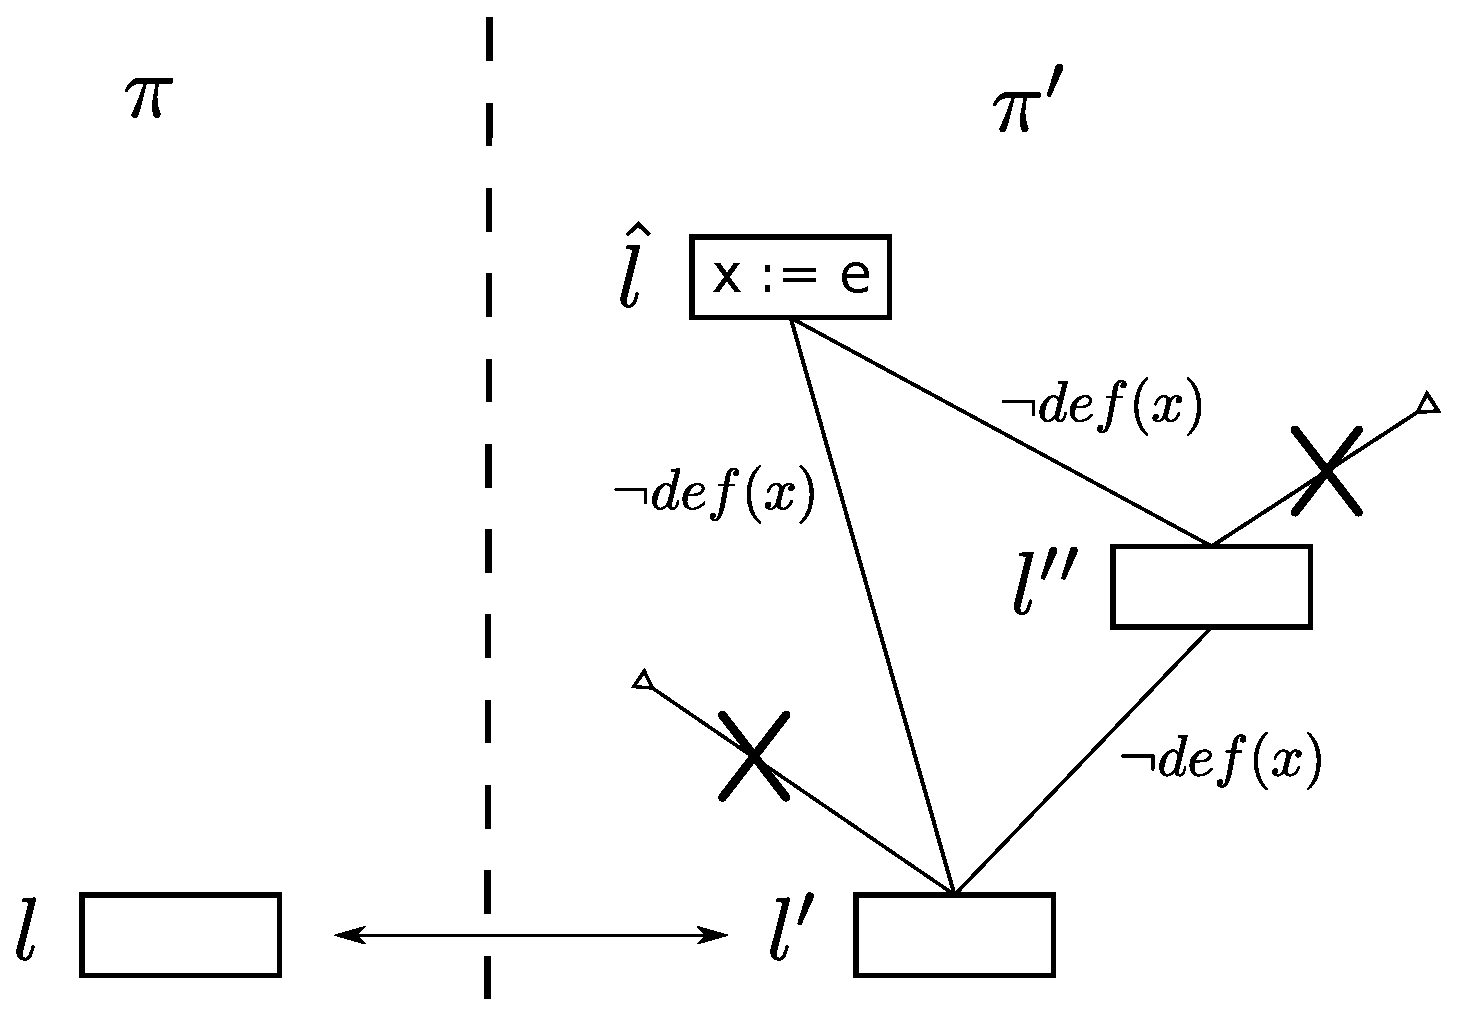
\includegraphics[width=0.49\textwidth]{figures/osr-reconstruct/osr-reconstruct.eps}
\caption{\protect\input{figures/osr-reconstruct/caption}}
\end{center}
\end{figure}
\fi

\begin{definition}[Live-Variable Equivalent Transformation]
\label{de:lve-trans}
A program transformation $T$ is {\em live-variable equivalent} (LVE) if for any program $\pi$, $\pi$ and $\mysem{T}(\pi)$ are live-variable bisimilar.
\end{definition}

\noindent We can finally establish the correctness of ${\tt OSR\_trans}$, which follows directly by \Cref{le:lvb-same-loc,le:build-comp-corr} and \ref{co:same-size}:

\begin{theorem}
\label{th:osr-trans-correctness}
For any program $\pi$ and live-variable equivalent transformation $T$, if ${\tt apply}(\pi,T)\triangleq(\pi', \Delta_I, \Delta_I)$ where $\pi'=\mysem{T}(\pi)$ and $\Delta_I:[1,|\pi|]\rightarrow [1,|\pi|]$ is the identity mapping between program points, then ${\tt OSR\_trans}(\pi,T)$ $=(\pi',\mu_{\pi\pi'},\mu_{\pi'\pi})$ yields a strict OSR mapping $\mu_{\pi\pi'}$ between $\pi$ and $\pi'$ and a strict OSR mapping $\mu_{\pi'\pi}$ between $\pi'$ and $\pi$.
\end{theorem}

\paragraph*{Discussion.} We remark that the assumption of an identity mapping between program points, which is a necessary condition of live-variable bisimilarity, is without loss of generality as it can  always be enforced by padding programs with \wskip\ statements. For instance, the Hoist transformation of \myfigure\ref{fig:sample-trans}, which we prove to be LVE in the next section, replaces the hoisted instruction with a \wskip, and expects a \wskip\ to already exist at the point where it is moved. As we discuss in \mysection\ref{ss:BC-implementation}, this is not required in a real compiler, as a transformation pass can be instrumented to capture code modifications that require updating the mapping.

\subsubsection{Examples of LVE Transformations}

\label{ss:lve-trans}

In this section, we show that classic compiler optimizations such as constant propagation, dead code elimination, and code hoisting as defined in \myfigure\ref{fig:sample-trans} are all examples of live-variable equivalent transformations. Hence, they are provably correct building blocks of an OSR-aware compilation toolchain based on algorithm $\osrtrans$. These optimizations are representatives of a broad class of transformations that insert, delete, and modify instructions. Further optimizations, which we do not formally discuss in this paper, are evaluated in \missing.

\begin{theorem}
\label{th:lve-trans-examples}
Transformations CP, DCE, and Hoist of \myfigure\ref{fig:sample-trans} are live-variable equivalent.
\end{theorem}

\begin{myproof}
\missing
In \cite{Lacey04}, CP, DCE, and Hoist are proven correct, each using a different bisimulation relation $R$. We propose a unifying approach based on live-variable bisimilarity. Let $\theta$ be a substitution that bounds free meta-variables with concrete program objects so that a rule's side-condition is satisfied. For CP, $R$ is the identity relation, hence $A(l)=Val\supseteq \live(\pi,l)\cap \live(\pi',l)$ in \mydefinition\ref{de:state-equiv-relation}. In DCE, $R$ is the identity relation before the eliminated assignment \mytt{x:=e}, and $A(l)=Val\setminus\{\theta(\wx)\}=\live(\pi,l)\cap \live(\pi',l)$ after it. For Hoist, $R$ is the identity relation before $\theta(p)$ and after $\theta(q)$ (see \myfigure\ref{fig:sample-trans}), and $A(l)=Val\setminus\{\theta(\wx)\}=\live(\pi,l)\cap \live(\pi',l)$ between them.
\end{myproof}
\subsubsection{Composing Multiple Transformation Passes}
\label{ss:trans-compose}

In this section, we show that OSR mappings can be composed, allowing several optimization passes to be applied to a program using algorithm ${\tt OSR\_trans}$. The first ingredient is {\em program composition}, defined as follows:

\begin{definition}[Program composition]
\label{de:composition}
We say that two programs $\pi,\pi'\in Prog$ with $\pi=\langle I_1,\ldots,I_n\rangle$ and $\pi'=\langle I'_1,\ldots,I'_{n'}\rangle$ are {\em composable} if $I_n=\texttt{out}~v_1,\ldots,v_k$ and $I'_1=\texttt{in}~v'_1,\ldots,v'_{k'}$ with $\{v'_1,\ldots,v'_{k'}\}\subseteq\{v_1,\ldots,v_k\}$. For any pair of composable programs $\pi,\pi'$, we define $\pi\circ\pi'=\langle I_1,\ldots,I_{n-1},\hat{I'}_2,\ldots,\hat{I'}_{n'}\rangle$, where $\forall i\in[1,n']$, $\hat{I'}_i$ is obtained from $I'_i$ by relocating each {\tt goto} target $m$ with $m+n-2$.
\iffalse
where $\chi\circ\chi'=\chi\setminus\{{\tt out \ldots}\}\cdot\chi'\left[
\begin{tiny}
\begin{array}{l}
\texttt{goto}~m\mapsto \\
\texttt{goto}~m+|\chi|-2
\end{array}
\end{tiny}
\right]\setminus\{{\tt in \ldots}\}$. 
\fi
\end{definition}

\begin{lemma}[Semantics of program composition]
\label{le:prog-comp-sem}
Let $\pi,\pi'\in Prog$ be any pair of composable programs, then $\forall\sigma\in\Sigma,$ $\mysem{\pi\circ\pi'}(\sigma)=\mysem{\pi'}\left(\mysem{\pi}(\sigma)\right)$.
\end{lemma}
\begin{myproof}
Straightforward by~\Cref{de:program-semantics,de:composition}.
\end{myproof}

\noindent We show how to define a composition of OSR mappings and we prove that it yields a valid OSR mapping.

\begin{lemma}[Mapping Composition]
\label{le:osr-mapping-comp}
Let $\pi,\pi',\pi''\in Prog$, let $\mu_{\pi\pi'}$ and $\mu_{\pi'\pi''}$ be OSR mappings as in \mydefinition\ref{de:osr-mapping}, and let $\mu_{\pi\pi'}\circ\mu_{\pi'\pi''}$ be a {\em composition of mappings} defined as follows:
\begin{gather*}
\forall l\in dom(\mu_{\pi\pi'})~s.t.~\mu_{\pi\pi'}(l)=(l',\chi)\wedge l'\in dom(\mu_{\pi'\pi''}):\\
\mu_{\pi'\pi''}(l')=(l'',\chi')\implies(\mu_{\pi\pi'}\circ\mu_{\pi'\pi''})(l)=(l'',\chi\circ\chi')
\end{gather*}
Then $\mu_{\pi\pi'}\circ\mu_{\pi'\pi''}$ is an OSR mapping from $\pi$ to $\pi''$.
\end{lemma}

\begin{myproof} 
Let $\mu_{\pi\pi''}=\mu_{\pi\pi'}\circ\mu_{\pi'\pi''}$. By \mydefinition\ref{de:osr-mapping}, it holds:
\begin{small}
\begin{gather*}
\forall \sigma\in\Sigma, \forall s_i=(\sigma_i,l_i)\in\tau_{\pi\sigma}~\text{s.t.}~l_i\in dom(\mu_{\pi\pi''}),\\
\exists \sigma',\sigma''\in\Sigma,~\exists s_j=(\sigma_j,l_j)\in\tau_{\pi'\sigma'}, \\ \exists s_k=(\sigma_k,l_k)\in\tau_{\pi''\sigma''}~\text{s.t.}~
\mu_{\pi\pi''}(l_i)=(l_k,\chi\circ\chi')~\wedge~\\ \mysem{\chi\circ\chi'}(\sigma_i\vert_{\live(\pi,l_i)})=\text{[by \ref{le:prog-comp-sem}]}\\
\mysem{\chi'}(\mysem{\chi}(\sigma_i\vert_{\live(\pi,l_i)}))=
\mysem{\chi'}(\sigma_j\vert_{\live(\pi',l_j)})=\sigma_k\vert_{\live(\pi'',l_k)}
\end{gather*}
\end{small}
Hence, $\mu_{\pi\pi'}\circ\mu_{\pi'\pi''}$ is an OSR mapping from $\pi$ to $\pi''$.
\end{myproof}

\begin{corollary}
\label{co:compose-strict}
Let $\pi,\pi',\pi''\in Prog$, let $\mu_{\pi\pi'}$ and $\mu_{\pi'\pi''}$ be strict OSR mappings as in \mydefinition\ref{de:osr-mapping}. Then $\mu_{\pi\pi'}\circ\mu_{\pi'\pi''}$ is a strict OSR mapping from $\pi$ to $\pi''$.
\end{corollary}
\begin{myproof}
Straightforward by \mydefinition\ref{de:osr-mapping} and \ref{le:osr-mapping-comp}.
\end{myproof}

\ifdefined\noauthorea
\begin{figure}[ht!]
\IncMargin{2em}
\begin{algorithm}[H]
\DontPrintSemicolon
\LinesNumbered
\SetAlgoNoLine
\SetNlSkip{1em} 
\Indm\Indmm
\hrulefill\\
\KwIn{Program $\pi$, list of program transformations $L$.}
\KwOut{Program $\hat{\pi}$, mappings $\mu_{\pi\hat{\pi}}$ and $\mu_{\hat{\pi}\pi}$.}
\nonl\vspace{-2mm}\hrulefill\\
\nonl$\mathbf{algorithm} \> \> \dopasses$($\pi$, $T::L$)$\rightarrow$($\pi''$, $\mu_{\pi\pi''}$, $\mu_{\pi''\pi}$):\;
\everypar={\nl}
\Indp\Indpp
\vspace{1mm} $(\pi',\mu_{\pi\pi'},\mu_{\pi'\pi})\gets \osrtrans(\pi,T)$\;
\lIf{$L=Nil$}{
    \Return{$(\pi',\mu_{\pi\pi'},\mu_{\pi'\pi})$}
}
$(\pi'',\mu_{\pi'\pi''},\mu_{\pi''\pi'})\gets \dopasses(\pi',L)$\;
\Return{$(\pi'',\mu_{\pi\pi'}\circ\mu_{\pi'\pi''},\mu_{\pi''\pi'}\circ\mu_{\pi'\pi})$}\;
\vspace{-2mm}
\Indm\Indmm
\nonl\hrulefill\vspace{1mm}\\
\DecMargin{2.5em}
\caption{\label{alg:osr-trans-compose} OSR-aware multi-pass program transformations.}
\IncMargin{2.5em}
\end{algorithm} 
\end{figure}

\else
\begin{figure}
\noindent
\begin{small}
\hphantom{xxx} $\textbf{algorithm}~{\tt do\_passes}(\pi, T::L)\rightarrow (\pi'',\mu_{\pi\pi''},\mu_{\pi''\pi})$ \\
1. ~~ ~~~~ $(\pi',\mu_{\pi\pi'},\mu_{\pi'\pi})\gets {\tt OSR\_trans}(\pi,T)$ \\
2. ~~ ~~~~ $\textbf{if}~L=Nil~\textbf{return}~ (\pi',\mu_{\pi\pi'},\mu_{\pi'\pi})$ \\
3. ~~ ~~~~ $(\pi'',\mu_{\pi'\pi''},\mu_{\pi''\pi'})\gets {\tt do\_passes}(\pi',L)$ \\
4. ~~ ~~~~ $\textbf{return}~(\pi'',\mu_{\pi\pi'}\circ\mu_{\pi'\pi''},\mu_{\pi''\pi'}\circ\mu_{\pi'\pi})$ \\
\end{small}
\caption{OSR-aware multi-pass program transformations.}
\label{alg:osr-trans-compose}
\end{figure}
\fi

\noindent Based on \ref{le:osr-mapping-comp}, we can easily prove by induction the correctness of the multi-pass transformation algorithm of \myalgorithm\ref{alg:osr-trans-compose}, which takes a program $\pi$ and a list of program transformations, and applies them to $\pi$, producing a bidirectional OSR mapping $\mu_{\pi\pi''},\mu_{\pi''\pi}$ between $\pi$ and the resulting program $\pi''$.
\subsection{Multi-Version Programs}

In this section, we propose a general OSR model where computations are described by a {\em multi-version program}, which consists of different versions of a program along with OSR mappings that allow execution to be transferred between them.

\begin{definition}[Multi-Version Program]
\label{de:mv-program}
A multi-version program is modeled by an edge-labeled graph $\Pi=({\cal V}, {\cal E}, {\cal M})$ where ${\cal V}=\{ \pi_1, \pi_2, \ldots,\pi_r\}$ is a set of program versions, ${\cal E}\subseteq \Pi^2$ is a set of edges such that $(\pi_p,\pi_q)$ indicates that an OSR transition can be fired from some point of $\pi_p$ to $\pi_q$,
%any point in $dom({\cal M}(\pi_i,\pi_j))$, 
and ${\cal M}:{\cal E}\rightarrow OSRMap$ labels each edge $(\pi,\pi')\in {\cal E}$ with an OSR mapping from $\pi$ to $\pi'$.
\end{definition}

\subsubsection{Semantics}

The state of a multi-version program is similar to the state of a program (\ref{de:prog-state}), but it also includes the index of the currently executed program version:

\begin{definition}[Multi-Version Program State]
The {\em state} of a multi-version program $\Pi=({\cal V}, {\cal E}, {\cal M})$ is described by a triple $(p,\sigma,l)$, where $p\in[1,|{\cal V}|]$ is the index of a program version, $\sigma$ is a memory store, and $l\in [1,|\pi_p|]$ is the point of the next instruction to be executed in $\pi_p$. The {\em initial state} from a store $\sigma$ is $(1,\sigma,1)$, i.e., computations start at $\pi_1$. We denote by $MState=\mathbb{N}\times\Sigma\times \mathbb{N}$ the set of all possible multi-version program states.
\end{definition}

\noindent The execution semantics of a multi-version program is described by the following transition relation:

\begin{definition}[Multi-Version Big-Step Transitions]
\label{de:osr-semantics}
For any multi-version program $\Pi$, relation $\Rightarrow_{\Pi}\subseteq MState\times MState$ is defined as follows:%, with meta-variables $\texttt{x}, \texttt{y}\in Var$, $\texttt{e}\in Expr$, and $\texttt{m}\in Num$:

\begin{footnotesize}
\begin{equation}
\label{eq:mv-big-step}
\begin{array}{rc}
(Norm)
&
\dfrac
{(\sigma, l)\Rightarrow_{\pi_p} (\sigma',l')}
{(p,\sigma, l)\Rightarrow_{\Pi} (p,\sigma',l')}
\\
\\
(OSR)
&
\dfrac
{(\pi_p,\pi_q)\in {\cal E} ~ \wedge ~ (l',\chi)={\cal M}(\pi_p,\pi_q)(l) ~ \wedge ~ \sigma'=\mysem{\chi}(\sigma)}
{(p,\sigma, l)\Rightarrow_{\Pi} (q,\sigma',l')}\\
\end{array}
\end{equation}
\end{footnotesize}
\end{definition}

\noindent The meaning is that at any time, execution can either continue in the current program version (Norm rule), or an OSR transition -- if possible at the current point -- can direct the control to another program version (OSR rule). The choice is non-deterministic, i.e., an oracle can tell the execution engine which rule to apply. In practice, the choice may be based for instance on profile data gathered by the runtime system: a common strategy is to dynamically ``OSR'' to the available version with the best expected performance on the actual workload. Notice that, since $\Rightarrow_{\Pi}$ may be non-deterministic, in general there may be different final stores for the same initial store. However, we are only interested in multi-version programs that deterministically yield a unique result, which guarantees semantic transparency of OSR transitions. 

\noindent To characterize the execution behavior of a multi-version program, we consider the system of traces of an execution transition system that start from a given initial state.

\begin{definition}[Trace System of Multi-Version Program]
\label{de:mvp-exec-system}
The system of traces ${\cal T}_{\Pi,\sigma}$ contains all traces $\tau$ of transition system $(MState,\Rightarrow_{\Pi})$ such that $\tau[0]=(1,\sigma,1)$.
\end{definition}

\begin{definition}[Deterministic Multi-Version Program]
\label{de:deterministic-mvp}
A multi-version program $\Pi$ is deterministic iff $\forall \sigma\in\Sigma$, either all traces in ${\cal T}_{\Pi,\sigma}$ are infinite, or they all lead to the same store, i.e.:
\begin{gather*}
\forall \tau, \tau'\in{\cal T}_{\Pi,\sigma}: ~~ \big(|\tau|=\infty ~ \Longleftrightarrow ~ |\tau'|=\infty\big) ~ \wedge \\
\big(|\tau|<\infty ~ \Longrightarrow ~ \exists~p,p',l,l'\in\mathbb{N}, \sigma,\sigma'\in\Sigma: ~ \\
\tau[|\tau|]=(p,\sigma,l) ~ \wedge ~ \tau'[|\tau'|]=(p',\sigma',l') ~ \wedge ~ \sigma=\sigma' \big).
\end{gather*}
\end{definition}

\noindent The meaning of a deterministic multi-version program can be defined as follows:

\begin{definition}[Multi-Version Semantic Function]
\label{de:mv-program-semantics}
The semantic function $\mysem{\Pi}:\Sigma \rightarrow \Sigma$ of a deterministic multi-version program $\Pi$ is defined as: 
$$
%\forall \sigma\in\Sigma: ~~ \mysem{\Pi}(\sigma)=\sigma' ~~ \Longleftrightarrow ~~ (1,\sigma,1) \Rightarrow^{*}_{\Pi} (p,\sigma',|\pi_p|+1) ~ \}
\forall \sigma\in\Sigma: ~~ \mysem{\Pi}(\sigma)=\sigma' ~~ \Longleftrightarrow ~~ (1,\sigma,1) \Rightarrow^{*}_{\Pi} (p,\sigma',|\pi_p|+1)
$$
where $\Rightarrow^{*}_{\Pi}$ is the transitive closure of $\Rightarrow_{\Pi}$.
\end{definition}

\subsubsection{Generation Algorithm and Correctness}

A natural way to generate a multi-version program consists in starting from a base program $\pi_1$ and constructing a tree of different versions, where each version is derived from its parent by applying one or more transformations. Using this approach and procedure \dopasses\ described in \mysection\ref{ss:trans-compose}, it is straightforward to construct a multi-version program $\Pi=({\cal V}, {\cal E}, {\cal M})$ such that:
\vspace{-1mm}
\begin{align*}
(\pi_p,\pi_q)\in {\cal E} ~~ \Longleftrightarrow ~~ \exists L: ~ &{\tt do\_passes}(\pi_p,L)=(\pi_q,\mu,\mu') ~ \wedge ~ {\cal M}(\pi_p,\pi_q)=\mu ~~ \vee \\
&{\tt do\_passes}(\pi_q,L)=(\pi_p,\mu,\mu') ~ \wedge ~ {\cal M}(\pi_p,\pi_q)=\mu'
\end{align*}

\noindent To prove the correctness of this approach, we introduce a preliminary lemma and then use it to prove that a multi-version program built in this way is deterministic.

\begin{lemma}
\label{le:comp-lemma}
Let $\tau\in{\cal T}_{\Pi,\sigma}$ be an execution trace in the system of the traces for the multi-version program $\Pi$ $=({\cal V}, {\cal E}, {\cal M})$ constructed using \dopasses\ and LVE transformations, and let $\omega_1,\ldots,\omega_k$ be the indices of $\tau$ where an OSR transition has just occurred. Then $\forall i\in[1,k]$ there exists a state $(\hat{\sigma}_i,\hat{l}_i)$ in the trace of $\hat{\pi}_i=\pi_{p_{\omega_{i}}}$ starting from the initial store $\sigma$ such that $\hat{l}_i=l_{\omega_i}$ and $\hat{\sigma}_i\vert_{\live(\hat{\pi}_i,\hat{l}_i)}=\sigma_{\omega_i}\vert_{\live(\hat{\pi}_i,\hat{l}_i)}$.
\end{lemma}
\begin{myproof}
\missing
\end{myproof}

\begin{theorem}[Multi-Version Program Determinism]
\label{th:mv-prog-determ}
Let $\Pi$ $=({\cal V}, {\cal E}, {\cal M})$ be a multi-version program constructed using \dopasses\ and live-variable equivalent transformations. Then $\Pi$ is deterministic.
\end{theorem}

\begin{myproof}
To prove that $\Pi$ is deterministic, we need to show that, given any initial store $\sigma$ on which $\pi_1\in\Pi$ terminates on some final state $\sigma'=\mysem{\pi_1}(\sigma)$, any execution trace $\tau\in{\cal T}_{\Pi,\sigma}$ terminates with $\sigma'$.

Let $\omega_1,\ldots,\omega_k$ be the indices of $\tau$ where an OSR transition has just occurred, i.e., for any $i\in[1,k]$, state $\tau[\omega_i]$ is obtained from $\tau[\omega_i-1]$ by applying compensation code $\chi_{\omega_i-1}$ on store $\sigma_{\omega_i-1}$, which yields a store $\sigma_{\omega_i}$. The transition leads from a point $l_{\omega_i-1}$ in version $\pi_{p_{\omega_i-1}}$ to a point $l_{\omega_i}=l_{\omega_i-1}$ in version $\pi_{p_{\omega_{i}}}$ in $\Pi$. 

By \mylemma\ref{le:comp-lemma}, $\forall i\in[1,k]$ there exists a state $(\hat{\sigma}_i,\hat{l}_i)$ in the trace of $\hat{\pi}_i=\pi_{p_{\omega_{i}}}$ starting from the initial store $\sigma$ such that $\hat{l}_i=l_{\omega_i}$ and $\hat{\sigma}_i\vert_{\live(\hat{\pi}_i,\hat{l}_i)}=\sigma_{\omega_i}\vert_{\live(\hat{\pi}_i,\hat{l}_i)}$. Hence, since no OSR is fired after $\omega_k$, by \myequation\ref{eq:mv-big-step} it holds: 
\begin{equation*}
(\hat{\pi}_k,\sigma_{\omega_{k}},l_{\omega_{k}})\trans^*_{\Pi}(\hat{\pi}_k,\sigma',|\hat{\pi}_k|+1) \Longleftrightarrow (\sigma_{\omega_{k}},l_{\omega_{k}})\trans^*_{\hat{\pi}_k}(\sigma',|\hat{\pi}_k|+1)
\end{equation*}

\noindent We can then apply \Cref{le:only-live-count,le:comp-lemma} to write:
\begin{gather*}
(\sigma_{\omega_{k}},l_{\omega_{k}})\trans^*_{\hat{\pi}_k}(\sigma',|\hat{\pi}_k|+1) \Longleftrightarrow \\ 
(\sigma_{\omega_{k}}\vert_{\live(\hat{\pi}_k,l_{\omega_{k}})},l_{\omega_{k}})\trans^*_{\hat{\pi}_k}(\sigma',|\hat{\pi}_k|+1) \Longleftrightarrow \\
(\hat{\sigma}_k\vert_{\live(\hat{\pi}_k,\hat{l}_k)},\hat{l}_k)\trans^*_{\hat{\pi}_k}(\sigma',|\hat{\pi}_k|+1)
\end{gather*}

\noindent As $(\hat{\sigma}_k,\hat{l}_k)\in\tau_{\hat{\pi}_k\sigma}$, by \ref{le:only-live-count} necessarily $\sigma'=\mysem{\hat{\pi}_k}(\sigma)$. 
Given that all programs in $\Pi$ are semantically equivalent, we can conclude that $\mysem{\Pi}(\sigma)=\sigma'=\mysem{\hat{\pi}_k}(\sigma)=\mysem{\pi_1}(\sigma)$.
\end{myproof}




\subsection{LLVM Implementation}

\subsection{Discussion}
\chapter{Experiments}

\section{HCCT Construction and Accuracy}

\section{{\em k-}iteration Path Profiling}

\section{On-Stack Replacement}
\chapter{Case Studies}
\label{ch:case-studies}

\section{Masked Convolution Filters in Image Processing}

\section{Optimizing Higher-Order Functions in MATLAB}
\chapter{Conclusions and Future Work}
\label{ch:conclusions}

We are confident that the ideas presented in this thesis can contribute to the advances in adaptive optimization technology for modern runtimes.

Collecting accurate profiling information with low overhead is a crucial factor for making online complex optimizations practical. In \mychapter\ref{ch:profiling} we have presented two analysis techniques that rely on elegant algorithmic solutions to profile data coming at a high rate from a large universe.

Our inter-procedural profiling technique enables the identification of most frequently encountered calling contexts without having to maintain the whole calling context tree in main memory - which we show can be impractical for real-world applications. We propose a compact data structure, the Hot Calling Context Tree (HCCT), that can be constructed thanks to the adoption of efficient data streaming algorithms. These algorithms provide us with strong theoretical guarantees on the accuracy and the space requirements of the solution, and operate with a constant per-item processing time.

Our intra-procedural profiling technique extends the well-known Ball-Larus algorithm to cyclic path profiles, in order to yield more optimization opportunities. We show that cyclic paths can be represented as concatenations of acylic Ball-Larus paths, and that a prefix forest can compactly encode them. We then introduce an intermediate data structure, the $k$-slab forest (\ksf), that can be constructed online with a constant per-item processing time and converted to a prefix forest on demand.

The algorithms behind our two profiling techniques have been implemented in mainstream systems and evaluated against prominent benchmarks. Theoretical guarantees are thus backed by promising experimental results, showing that our techniques can be used in practical scenarios where previous solutions failed.

In \mychapter\ref{ch:continuous} we have then focused our attention on another main player of adaptive optimization cycles, On-Stack Replacement (OSR), which enables runtimes to divert the execution to freshly generated optimized code using profiling information, or to deoptimize to a different version of the code when conditions change, e.g., when program's behavior starts to diverge from the profile significantly.

OSR is not only a great engineering problem, but also an intellectually challenging endeavor. We thus tackle the problem from both a practical and theoretical perspective. We present a new framework for on-stack replacement that combines some of the best practices observed in literature, such as platform independence and the generation of highly optimized continuation functions, with two novel features: the ability to perform OSR at any program location, and a compensation code abstraction to encode changes to the program state, thus increasing the flexibility of OSR itself. Experimental results collected on classic benchmarks for our \osrkit\ embodiment in the LLVM compiler toolchain suggest that encoding OSR at intermediate representation level allows the compiler to generate very efficient machinery with a hardly noticeable impact on performance. As the ideas behind our OSR framework are general, we do not foresee any limitation to its adoption in other runtime environments as well.

In the second part of \mychapter\ref{ch:continuous}, we then make a first attempt to prove OSR transitions sound. To capture OSR in its full generality, we define a notion of multi-program, and let an oracle decide at each program step in which version of the multi-program execution should continue. We distill the essence of OSR to a simple imperative calculus with an operational semantics. Using program bisimulation, we prove that an OSR can correctly divert execution across program versions if they have been generated applying live-variable equivalent transformations. We also present an algorithm that can relieve code optimizers from the burden of generating all the required glue machinery to realign the state during an OSR transition.

There is a trade-off between the number of points where OSR can be correctly fired and the price to pay in terms of space and time in order to support them. Our work lies at the performance-preserving end of the spectrum, supporting OSR transitions in constant time and space. The approach we propose does not impose any barriers to optimizations, which run unhindered, and does not require any state logging. To assess the practical impact of this design choice, we analyze experimentally the fraction of program locations where OSR can be efficiently fired in prominent benchmarks across several LLVM optimization passes. Our experiments suggest that bidirectional OSR transitions between rather different program versions can be supported almost everywhere in the code, under several classic optimizations.

Finally, we present a number of case studies as examples of the end-to-end utility of the techniques described in this thesis. All of our code is publicly available and, for \kblpp\ and \osrkit, it has been endorsed along with the associated experiments by Artifact Evaluation processes of known conferences on programming languages.

\section*{Future Work}
The methodologies and ideas presented in this thesis leave a number of interesting open questions that we hope to address in future work.

We believe that a careful use of data mining techniques has the potential benefit of enabling some previously impossible dynamic program analysis tasks, which would otherwise be too costly. In particular, our techniques could be applied to certain forms of path profiling: e.g., they could help leverage the scalability problems encountered when collecting performance metrics about interprocedural paths (i.e., acyclic paths that may cross procedure boundaries)~\cite{Melski99}.

\backmatter

\bibliographystyle{abbrvnat}
\bibliography{bibliography/biblio.bib}

\end{document}